%! Author = Omar Iskandarani
%! Title = The Vortex Æther Model: A Unified Topological Field Theory of Mass, Gravity, and Time
%! Date = ...
%! Affiliation = Independent Researcher, Groningen, The Netherlands
%! License = CC BY-NC 4.0
%! ORCID = 0009-0006-1686-3961
%! DOI = 10.5281/zenodo.15848011


\newcommand{\paperdoi}{10.5281/zenodo.15848011}
\documentclass[preprint]{revtex4-2}

% ==================== Packages ====================
\usepackage[utf8]{inputenc}
\usepackage[T1]{fontenc}
\usepackage{lmodern}
\usepackage{amsmath,amssymb,amsfonts}
\usepackage{graphicx}
\usepackage{hyperref}
\usepackage{doi}
\usepackage{physics}
\usepackage{mathtools}
\usepackage{tikz}
\usetikzlibrary{knots,intersections,decorations.pathreplacing}
\usetikzlibrary{3d, calc, arrows.meta, positioning}
\usepackage{pgfmath}
\usetikzlibrary{decorations.pathmorphing}
\usepackage{pgfplots}
\pgfplotsset{compat=1.18} % or version you have
\usepackage{bm}          % bold math
\usepackage{titlesec}    % section formatting (optional)
\usepackage{float}       % [H] float placement
\usepackage[font=footnotesize]{caption}

% ==================== Metadata ====================
\begin{document}

\title{The Vortex Æther Model: \\[1ex]
        \large A Unified Topological Field Theory of Mass, Gravity, and Time}

\author{Omar Iskandarani}
\email{info@omariskandarani.com}
\affiliation{Independent Researcher, Groningen, The Netherlands}
\thanks{ORCID: \href{https://orcid.org/0009-0006-1686-3961}{0009-0006-1686-3961}}
\thanks{DOI: \href{https://doi.org/\paperdoi}{\paperdoi}}
\thanks{License: CC BY-NC 4.0 International}

\date{\today}

% ==================== Abstract ====================
\begin{abstract}
            We present the Vortex Æther Model (VAM), a unified physical framework in which mass, gravity, and proper time emerge from topologically structured vorticity within a compressible, inviscid æther. In contrast to curvature-based relativity and Higgs-based mass generation, VAM describes particles as knotted vortex excitations, and gravity as a swirl-induced time deviation field. The theory reproduces classical phenomena such as gravitational redshift, time dilation, and frame-dragging through fluid-dynamic energetics, and calculates particle masses and physical constants from first principles. The Standard Model gauge groups SU(3), SU(2), and U(1) arise naturally from vortex topology and swirl symmetry, while canonical quantization defines a Fock-like Hilbert space over knot eigenstates. We develop a full path-integral formulation over topological sectors of the æther manifold, enabling quantum transitions, knot fusion, and helicity exchange interactions. Benchmarking against general relativity and experimental tests of gravitational time deviation support the model’s viability. VAM offers a physically grounded, falsifiable, and derivational alternative to conventional quantum gravity and field theory models.\\
            \begin{center}
            VAM Used Knots:\\
            \( Unknot \):~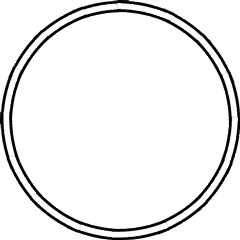
\includegraphics[height=1.2em]{images/0_1} Photon \\
            \( Hopf link \):~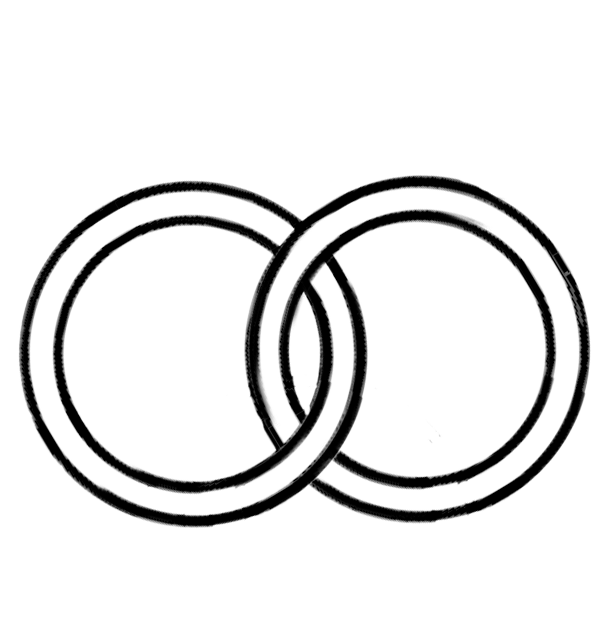
\includegraphics[height=1.2em]{images/hopf} Massive Boson / Polariton \( Solomon \):~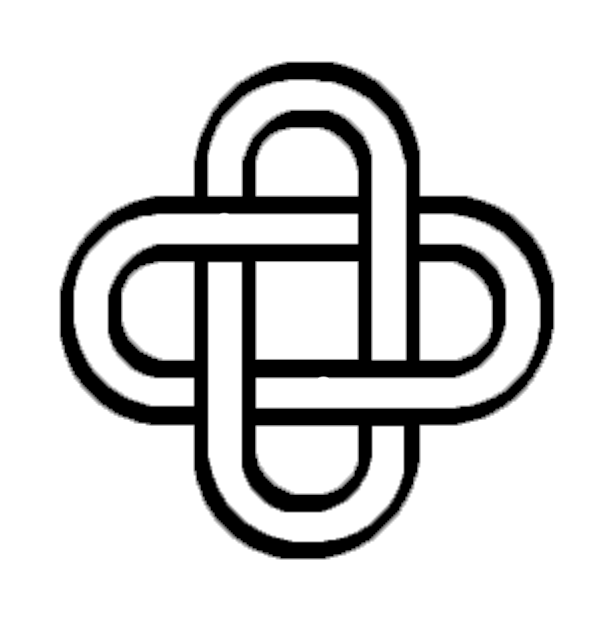
\includegraphics[height=1.2em]{images/solomon} Electron / Positron\\
            \( Borromean \):~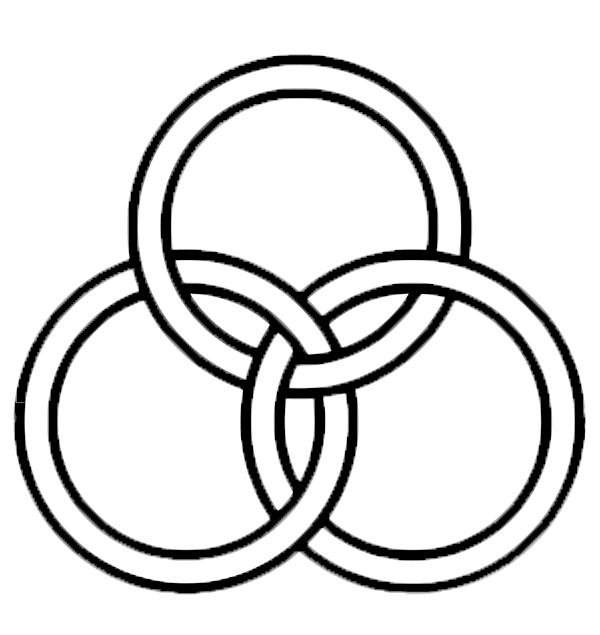
\includegraphics[height=1.2em]{images/borromean} Proton \( Trefoil Knot (3,2) \):~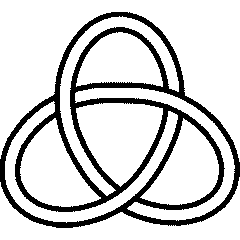
\includegraphics[height=1.2em]{images/3_1} Neutrino \\
            \( 6_2 \):~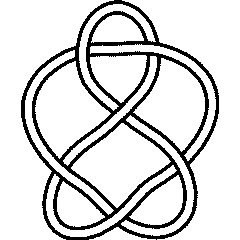
\includegraphics[height=1.2em]{images/6_2} Up-Quarck \( 7_4 \):~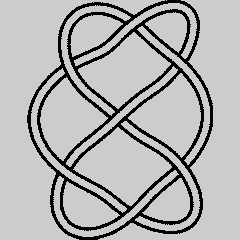
\includegraphics[height=1.2em]{images/7_4} Down-Quarck  \\
            \( Figure-8-knot \):~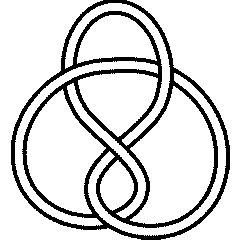
\includegraphics[height=1.2em]{images/4_1} Dark Matter / Energy
\begin{tikzpicture}[scale=0.1,  line width=0.4pt]
  \def\nsamples{60}
  \foreach \i in {1,...,\nsamples} {
      \pgfmathsetmacro\tprev{(\i - 1) * 2 * pi / \nsamples}
      \pgfmathsetmacro\tcurr{\i * 2 * pi / \nsamples}
      \pgfmathsetmacro\xprev{(2 + cos(2 * \tprev r)) * cos(3 * \tprev r)}
      \pgfmathsetmacro\yprev{(2 + cos(2 * \tprev r)) * sin(3 * \tprev r)}
      \pgfmathsetmacro\xcurr{(2 + cos(2 * \tcurr r)) * cos(3 * \tcurr r)}
      \pgfmathsetmacro\ycurr{(2 + cos(2 * \tcurr r)) * sin(3 * \tcurr r)}
      \draw[black, --] (\xprev,\yprev) -- (\xcurr,\ycurr);
  }
\end{tikzpicture}\\
 \( 5_1 \):~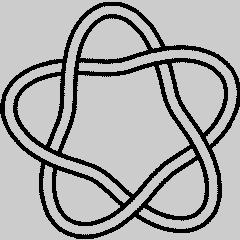
\includegraphics[height=1.2em]{images/5_1}
 \( 5_2 \):~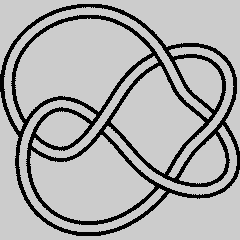
\includegraphics[height=1.2em]{images/5_2}
 \( 7_2 \):~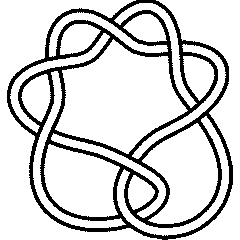
\includegraphics[height=1.2em]{images/7_2}
\end{center}
\end{abstract}
\maketitle

% ==================== Table of Contents (optional) ====================
\newpage
\begingroup
\setlength{\baselineskip}{0.9\baselineskip}  % Adjust this factor as needed
\tableofcontents
\endgroup
\vspace{1em}
\newpage
% ============= Begin of content ============
\section{Introduction and Motivation}\label{sec:introduction-and-motivation}
    The quest for a unified framework of fundamental physics remains unresolved. While General Relativity (GR) provides a powerful geometric description of gravity~\cite{einstein1915gr}, and the Standard Model (SM) successfully accounts for particle interactions via gauge symmetries~\cite{weinberg1995quantum}, these theories are conceptually and structurally incompatible. GR is formulated as a smooth, four-dimensional Riemannian geometry with dynamical curvature, while the SM operates on flat spacetime with point particles, quantum fields, and externally imposed mass via the Higgs mechanism.

    Despite their predictive power, both frameworks leave foundational questions unanswered:
    \begin{itemize}
        \item What is the origin of inertial mass, beyond spontaneous symmetry breaking?
        \item Why does proper time slow near massive bodies, and can this be described without spacetime curvature?
        \item What underlying physical structure connects gravitation, mass-energy, and quantum phase?
        \item Can the values of fundamental constants (e.g., $G$, $\alpha$, $\hbar$) be derived, rather than inserted?
    \end{itemize}

    The \textbf{Vortex \AE ther Model (VAM)} offers a new ontological starting point. It describes the universe as a structured, compressible, inviscid fluid---a physical \ae ther---embedded in a 3D Euclidean manifold with an absolute æther time $N$. Within this medium, particles are not pointlike but are stable \textit{topological knots} in the vorticity field. Mass, proper time, and gravitational attraction arise from swirl energetics, helicity density, and the emergent dynamics of local vortex configurations.

    This approach does not invoke curvature or external scalar fields; instead, it derives time deviation, gravitational pressure, and inertial resistance from first principles in topological fluid mechanics. By defining a swirl scalar potential $\Phi(\vec{x},t)$, a velocity field $\vec{v} = \nabla \Phi$, and a vorticity field $\vec{\omega} = \nabla \times \vec{v}$, the theory reconstructs gravity as a time-dilating flow field and quantizes particles as eigenmodes of knotted circulation.

    VAM builds on and surpasses prior analog models of gravity (e.g., superfluid vacuum theory~\cite{barcelo2011analogue}, analog BEC spacetimes~\cite{volovik2003universe}), but extends them into a complete field theory. It defines a Standard Model Lagrangian in terms of vortex knots and swirl symmetries, derives the values of $m_e$, $G$, and $\alpha$ from vortex geometry, and introduces a full canonical quantization scheme over a Hilbert space of knot eigenstates. It also aligns naturally with emergent gravity models like those of Jacobson~\cite{jacobson1995thermo} and Verlinde~\cite{verlinde2011emergent}, while offering a mechanical substrate and observable predictions.

    This paper presents the full structure of the Vortex \AE ther Model, from its ontological foundations and swirl dynamics to its quantized field theory, Standard Model reconstruction, and experimental predictions.

\section{Ontological Foundations: Æther, Swirl, and Time}\label{sec:ontological-foundations:-ther-swirl-and-time}
    The Vortex \AE ther Model (VAM) is grounded in a physically realist ontology: the universe is composed of a compressible, inviscid fluid medium known as the \ae ther, embedded in a flat 3-dimensional Euclidean manifold $\mathbb{E}^3$ and parameterized by an absolute scalar time $N$. This æther forms the continuous substrate for all dynamics, structure, and causality. Swirl clocks $S(t)$ serve as the intrinsic timekeeping mechanisms for vortex-bound particles, representing a helicity-driven deviation from both proper time $\tau$ and global æther time $N$.

    \subsection{The Æther Manifold $\mathcal{N}$ and Temporal Embedding}
    We define the spacetime substrate as a 4-dimensional manifold $\mathcal{N} = \mathbb{E}^3 \times N$, where $N$ is the global æther time. All fields in VAM are defined over $\mathcal{N}$. Unlike in General Relativity, spacetime is not dynamical; instead, all physical dynamics arise from internal structure in the æther's flow fields. This allows for absolute simultaneity in æther time, while local time experiences can vary depending on vortex structures.

    \subsection{Swirl Fields and Scalar Potentials}
    The central dynamic quantity in VAM is the swirl scalar potential $\Phi(\vec{x},t)$, from which the velocity field is defined as:
    \begin{equation}
        \vec{v} = \nabla \Phi
        \label{eq:velocity_from_potential}
    \end{equation}
    This is standard in vortex filament theory~\cite{saffman1992vortex} and classical fluid dynamics~\cite{batchelor2000introduction}.
    The vorticity field is then given by:
    \begin{equation}
        \vec{\omega} = \nabla \times \vec{v}
        \label{eq:vorticity_definition}
    \end{equation}
    These fields describe structured circulations and knots within the æther. Swirl configurations evolve over æther time $N$, and contain energy, helicity, and proper time deviation.

    \subsection{Temporal Ontology: Proper Time and Swirl Clocks}
    VAM introduces a layered model of time:
    \begin{itemize}
        \item \textbf{Æther Time \boldsymbol\(N\):} The global, absolute temporal parameter of the manifold $\mathcal{N}$
        \item \textbf{Proper Time \boldsymbol\(\tau\):} The time experienced by a particle or knot, delayed by swirl-induced time deviation
        \item \textbf{Swirl Clock Phase \boldsymbol\(S(t)\):} A local temporal field defined by helicity density $(\vec{v} \cdot \vec{\omega})$
        \item \textbf{Vortex Proper Time \boldsymbol\(T_v\):} A phase cycle variable associated with the internal twist of a vortex knot
    \end{itemize}

    Gravitational time dilation is thus an emergent phenomenon: when swirl velocity increases, proper time slows as:
    \begin{equation}
        \frac{d\tau}{dN} = \sqrt{1 - \frac{v^2}{c^2}}
        \label{eq:basic_time_deviation}
    \end{equation}
    This generalizes to:
    \begin{equation}
        \frac{d\tau}{dN} = \sqrt{1 - \frac{(\vec{v} \cdot \vec{\omega})^2}{\omega_{\text{bg}}^2 c^2}}
        \label{eq:helicity_time_deviation}
    \end{equation}
    in the presence of background swirl fields. These relations reproduce the classical effects of redshift, gravitational delay, and relativistic contraction without invoking spacetime curvature.

    \subsection{Knot Causality and Topological Stability}
    Particles in VAM are not points, but stable, knotted configurations in the vorticity field. Each knot type $K_{p,q}$ (e.g., trefoil, torus, hyperbolic) defines a causally persistent structure with intrinsic energy, tension, and helicity~\cite{moffatt1969degree, arnold1998topological}. These knots evolve in the manifold $\mathcal{N}$ and obey conservation of circulation $\Gamma$ and linking number $Lk$ under ideal fluid flow. Their motion is governed by Eulerian advection and vortex filament equations.

    \subsection*{Summary: Physical Ontology of VAM}
    VAM replaces the postulates of field and curvature with:
    \begin{itemize}
        \item A real, compressible fluid medium — the æther — as the basis of reality;
        \item Topological structures in swirl fields as the origin of particles, mass, and interaction;
        \item Time as a multi-modal, emergent experience derived from flow, helicity, and phase;
        \item Gravity as a fluid-dynamic phenomenon: structured swirl replaces curved geometry.
    \end{itemize}

\section{Swirl Kinematics and Classical Gravitation}\label{sec:swirl-kinematics-and-classical-gravitation}
    In the Vortex \AE ther Model (VAM), gravity is not described by spacetime curvature but emerges from pressure gradients and time deviation in a structured swirl field. Gravitational phenomena arise from variations in the flow speed, helicity, and vorticity of the æther, modeled as a compressible, inviscid fluid. This section derives classical gravitational effects—such as redshift, time dilation, and orbital acceleration—from swirl dynamics and vortex energetics.

    \subsection{Swirl Field Velocity and Time Deviation}
    The swirl velocity field is defined as in Eq.~\ref{eq:velocity_from_potential}, with corresponding vorticity from Eq.~\ref{eq:vorticity_definition}. Proper time deviation follows Eq.~\ref{eq:basic_time_deviation}, which expresses how local swirl speed delays proper time $\tau$ relative to global æther time $N$.

    This expression recovers the Schwarzschild time dilation formula when the swirl velocity is azimuthal, i.e., $v = v_\phi(r)$, as around a stationary massive source.

    \subsection{Gravitational Redshift from Swirl Clock Phase}
    The local swirl clock phase $S(t)$ evolves with helicity density, and redshift between an emitter and observer is:
    \begin{equation}
        \frac{f_{\text{emit}}}{f_{\text{obs}}} = \sqrt{1 - \frac{v_{\text{emit}}^2}{c^2}} \bigg/ \sqrt{1 - \frac{v_{\text{obs}}^2}{c^2}}
        \label{eq:gravitational_redshift}
    \end{equation}

    This has the same functional form as classical gravitational redshift but arises from fluidic swirl energy instead of spacetime metric potentials.

    \subsection{Frame-Dragging as Vortex Coupling}
    Nearby test particles experience rotational acceleration from background swirl gradients:
    \begin{equation}
        \vec{a}_\theta = \Gamma \frac{\partial \vec{\omega}}{\partial r}
        \label{eq:frame_drag_accel}
    \end{equation}
    This mimics Lense–Thirring frame dragging as an emergent property of circulation coupling~\cite{thorne1986blackholes}.

    \subsection{Inertial Mass from Swirl Resistance}
    VAM proposes that inertial mass arises from the local swirl energy stored in the vorticity field. The swirl energy of a region $\mathcal{V}$ is:
    \begin{equation}
        E_{\text{swirl}} = \frac{1}{2} \rho_{\text{\ae}}^{\text{(mass)}} \int_{\mathcal{V}} |\vec{\omega}|^2 \, d^3x
        \label{eq:swirl_energy}
    \end{equation}

    The inertial mass is then:
    \begin{equation}
        m_{\text{inertial}} = \frac{E_{\text{swirl}}}{c^2}
        \label{eq:inertial_mass}
    \end{equation}

    This realizes the Machian principle locally: resistance to acceleration arises from momentum-storing swirl structures, not from spacetime geometry.

    \subsection{Recovery of Newtonian and Relativistic Limits}
    In low-vorticity and low-velocity limits, swirl pressure gradients obey a Bernoulli-type equation:
    \begin{equation}
        \frac{1}{2} \rho v^2 + p + \rho \Phi_g = \text{const.}
        \label{eq:bernoulli_grav}
    \end{equation}

    This leads to a classical gravitational force:
    \begin{equation}
        \vec{F}_g = -m \nabla \Phi_g
        \label{eq:newtonian_grav_force}
    \end{equation}

    In analogy with Newton–Poisson gravity, we interpret the swirl-induced gravitational potential \( \Phi \) as satisfying:
    \begin{equation}
        \nabla^2 \Phi(\vec{x}) = - \frac{1}{2} \lambda_g |\vec{\omega}(\vec{x})|^2
        \label{eq:swirl_poisson}
    \end{equation}

    This shows that vorticity density acts as the source of gravitational potential in VAM.

    Under high swirl conditions, the full relativistic proper time deviation re-emerges as:
    \begin{equation}
        \frac{d\tau}{dN} = \sqrt{1 - \frac{\omega^2 r^2}{c^2}}
        \label{eq:general_swirl_time}
    \end{equation}

    \subsection{Benchmarking Against GR}
    This formulation reproduces:
    \begin{itemize}
        \item Time dilation near rotating bodies (e.g., GPS satellites, pulsars)
        \item Gravitational redshift and lensing (via pressure gradients and swirl density)
        \item Frame-dragging effects (via circulation field gradients)
    \end{itemize}
    These effects have been validated numerically in the VAM benchmarking study~\cite{vam_benchmark2025}.


\section{Particles as Vortex Knots — Mass and Topology}
    The Vortex \AE{}ther Model (VAM) interprets all elementary particles, atoms, and molecules as quantized vortex knots in an inviscid, compressible fluid-like medium. These knotted configurations carry energy, chirality, and linking number, and evolve through the distinct temporal modes defined earlier: global æther time \( N \), vortex proper time \( T_v \), swirl phase time \( S(t) \), and observer time \( \tau \). This topological ontology builds on classic work in vortex dynamics~\cite{moffatt1969degree, arnold1998topological, saffman1992vortex} and recent laboratory creation of knotted quantum vortices~\cite{kleckner2013creation}.

    \subsection{Knot-Based Particle Taxonomy}
        \begin{figure}[H]
            \centering
            \footnotesize
            \scalebox{0.75}{
                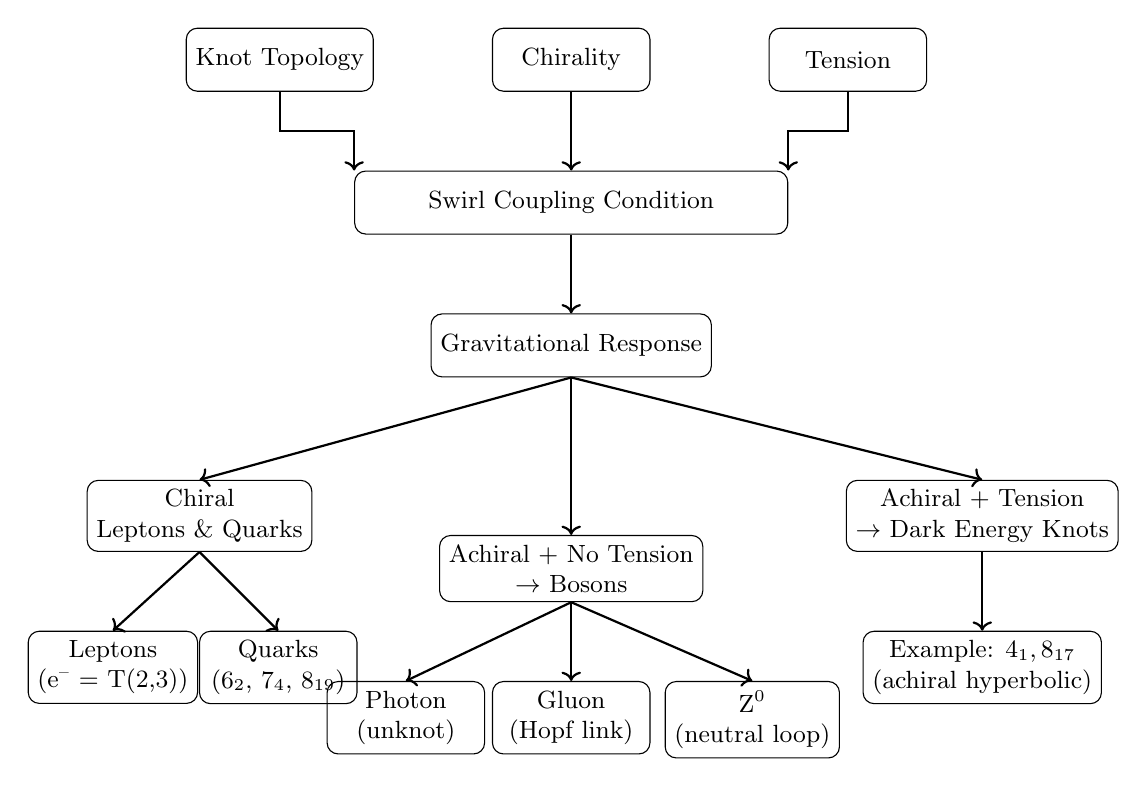
\begin{tikzpicture}[
                  box/.style = {draw, rounded corners, minimum width=2.0cm, minimum height=0.8cm, font=\small, align=center},
                  arrow/.style = {->, thick},   node distance=1.0cm and 1.5cm
                ]
                    % Inputs
                    \node[box] (topology) {Knot Topology};
                    \node[box, right=of topology] (chirality) {Chirality};
                    \node[box, right=of chirality] (tension) {Tension};

                    % Swirl coupling
                    \node[box, below=of chirality, minimum width=5.5cm] (coupling) {Swirl Coupling Condition};

                    % Gravitational response
                    \node[box, below=of coupling] (grav) {Gravitational Response};

                    % Gravitational classes
                    \node[box, below left=1.3cm and 1.5cm of grav] (matter) {Chiral\\Leptons \& Quarks};
                    \node[box, below=2cm of grav] (boson) {Achiral + No Tension\\\(\rightarrow\) Bosons};
                    \node[box, below right=1.3cm and 1.7cm of grav] (dark) {Achiral + Tension\\\(\rightarrow\) Dark Energy Knots};

                    % Subclasses
                    \node[box, below=of matter, xshift=-1.1cm] (leptons) {Leptons\\(e\textsuperscript{--} = T(2,3))};
                    \node[box, below=of matter, xshift=+1.0cm] (quarks) {Quarks\\(6\textsubscript{2}, 7\textsubscript{4}, 8\textsubscript{19})};

                    \node[box, below=of boson, xshift=-2.1cm] (photon) {Photon\\(unknot)};
                    \node[box, below=of boson] (gluon) {Gluon\\(Hopf link)};
                    \node[box, below=of boson, xshift=+2.3cm] (zboson) {Z\textsuperscript{0}\\(neutral loop)};

                    \node[box, below=of dark] (darkex) {Example: \(4_{1}, 8_{17}\)\\ (achiral hyperbolic)};

                    % Arrows to coupling
                    \draw[arrow] (topology.south) -- ++(0,-0.5) -| (coupling.north west);
                    \draw[arrow] (chirality.south) -- (coupling.north);
                    \draw[arrow] (tension.south) -- ++(0,-0.5) -| (coupling.north east);

                    % Arrows down flow
                    \draw[arrow] (coupling.south) -- (grav.north);
                    \draw[arrow] (grav.south) -- (matter.north);
                    \draw[arrow] (grav.south) -- (boson.north);
                    \draw[arrow] (grav.south) -- (dark.north);

                    % Particle branches
                    \draw[arrow] (matter.south) -- (leptons.north);
                    \draw[arrow] (matter.south) -- (quarks.north);

                    \draw[arrow] (boson.south) -- (photon.north);
                    \draw[arrow] (boson.south) -- (gluon.north);
                    \draw[arrow] (boson.south) -- (zboson.north);

                    \draw[arrow] (dark.south) -- (darkex.north);
                \end{tikzpicture}
            }
            \caption{\footnotesize
            \textbf{Knot Classification by Swirl Coupling.}
                The flowchart visualizes how knot topology, chirality, and curvature tension determine gravitational behavior, and how this leads to specific particle subclasses:
                    \\ \textbf{Chiral knots} align with swirl fields and form matter: \textbf{leptons} (torus knots) and \textbf{quarks} (hyperbolic knots).
                    \\ \textbf{Achiral, tensionless} structures like unknots and Hopf links are \textbf{bosons}, passively guided by swirl tubes.
                    \\ \textbf{Achiral knots with tension} are expelled, forming \textbf{dark energy} candidates.
            }\label{fig:knot-classification}
        \end{figure}

    The classification of matter in VAM arises from knot type, chirality, and internal curvature tension. This generates a natural taxonomy:

    \begin{itemize}
        \item \textbf{Leptons:} Simple torus knots such as the left-handed trefoil \( T(2,3) \), corresponding to the electron.
        \item \textbf{Quarks:} Chiral hyperbolic knots with high helicity and tension (e.g., \( 6_2, 7_4 \)).
        \item \textbf{Bosons:} Achiral knots with negligible torsion. Examples: photon (unknot), gluon (Hopf link), \( Z^0 \) (neutral loop).
        \item \textbf{Dark Energy Candidates:} Achiral, high-tension hyperbolic knots (e.g., \( 4_1, 8_{17} \)) that are repelled by swirl field coherence.
    \end{itemize}

    The classification scheme is summarized visually in Fig.~\ref{fig:knot-classification}, which organizes particle types based on knot topology, chirality, and curvature tension.

    A full taxonomy of particle-associated vortex knots—including topological class, chirality, and mass behavior—is presented in Appendix~\ref{tab:knot_taxonomy}. This gravitational classifier refines earlier analogs using quantized vortex tubes~\cite{volovik2003universe} and topologically stable defects~\cite{ranada1992knots}.

    \subsection{Chirality, Time, and Matter-Antimatter Duality}
    In VAM, chirality is not superficial but defines the knot’s alignment with temporal flow:

    \begin{itemize}
        \item \textbf{Left-handed knots} align with the swirl clock \( S(t) \) and evolve forward in proper time \( T_v \): these correspond to matter.
        \item \textbf{Right-handed knots} evolve with reversed swirl phase: these correspond to antimatter.
    \end{itemize}

    Matter–antimatter asymmetry emerges from global æther vorticity, which biases toward one chirality sector, offering a topological basis for parity violation.

    \subsection{Swirl Energy and Charge from Helicity}
    The rest energy of a vortex knot arises from confined swirl motion:

    \begin{equation}
    E_{\text{knot}} = \frac{1}{2} \rho_{\text{\ae}}^{\text{(mass)}} C_e^2 \cdot V_{\text{knot}}
    \label{eq:raw_swirl_energy}
    \end{equation}

    Here \( \rho_{\text{\ae}}^{\text{(mass)}} \) is the mass-equivalent æther density~(see Appendix~\ref{sec:constants_derivation}), \( C_e \) is the characteristic swirl speed, and \( V_{\text{knot}} = V_i \cdot V_{\text{torus}} \) is the effective volume of the knotted structure.

    In addition to mass, the swirl configuration determines electric charge via helicity flux:

    \paragraph{Electric Charge as Æther Helicity Flux:}
    The electric field is modeled as a helicity flux sourced by swirl topology:

    \begin{equation}
        \vec{E}_{\text{\ae}} = \kappa \frac{H}{4\pi r^2} \hat{r}, \quad \text{where } H = \int \vec{v} \cdot \vec{\omega} \, d^3x
    \end{equation}

    Thus, electric charge is the conserved topological twist of a knot, and Coulomb’s law arises from vortex helicity gradients~\cite{ranada1992knots}.

    \subsection{Mass Formula with Topological Amplification}
    This raw energy is scaled by a topological amplification factor, which accounts for coherence and core structure:

    \begin{equation}
    M = \left( \frac{4}{\alpha \varphi} \right) \cdot \xi(n) \cdot \left( \frac{1}{2} \rho_{\text{\ae}}^{\text{(mass)}} C_e^2 \sum_i V_i \right)
    \label{eq:mass_formula_basic}
    \end{equation}

    Here \( \alpha \approx 1/137 \) is the fine-structure constant, and \( \varphi = \frac{1 + \sqrt{5}}{2} \approx 1.618 \) is the golden ratio. The coherence factor is:

    \begin{equation}
    \xi(n) = n^{-1/\varphi}
    \label{eq:coherence_factor}
    \end{equation}

    where \( n \) is the number of swirl cores forming the knot bundle.

    \subsection{Derived Baryon Masses}
    Baryons are modeled as composite knots of three subcores. Their masses are given by:

    \begin{align}
    M_p &= \frac{1}{\varphi^2} \cdot 3^{-1/\varphi} \cdot (2 M_u + M_d) \\
    M_n &= \frac{1}{\varphi^2} \cdot 3^{-1/\varphi} \cdot (M_u + 2 M_d)
    \end{align}

    with

    \begin{equation}
    M_{u,d} = \frac{4}{\alpha \varphi} \cdot \frac{1}{2} \rho_{\text{\ae}}^{\text{(mass)}} C_e^2 \cdot V_{u,d}
    \end{equation}

    and empirically calibrated core volumes:

    \begin{equation}
    V_u \approx 3.123 \times 10^{-43} \, \text{m}^3, \quad V_d \approx 3.494 \times 10^{-43} \, \text{m}^3
    \end{equation}

    These yield baryon masses accurate to within 1–2\% of observed values using only geometric and topological inputs~\cite{kleckner2013creation}.

    \subsection{Master Formula for All Knot-Based Masses}
    All particle masses are unified under a general formula:

    \begin{equation}
    M(n, m, \{V_i\}) = \left( \frac{4}{\alpha} \right) \cdot \left( \frac{1}{m} \right)^{3/2} \cdot \frac{1}{\varphi^s} \cdot n^{-1/\varphi} \cdot \sum_i V_i \cdot \left( \frac{1}{2} \rho_{\text{\ae}}^{\text{(mass)}} C_e^2 \right)
    \label{eq:mass_master}
    \end{equation}

    Where:
    \begin{itemize}
        \item \( n \): number of vortex cores,
        \item \( m \): winding thread count,
        \item \( s \): topological suppression index (e.g., 0–3),
        \item \( V_i \): core volumes of constituent subknots.
    \end{itemize}

    \noindent Representative examples:
    \begin{itemize}
        \item Electron: \( n=1, m=1, s=0 \)
        \item Proton: \( n=3, m=1, s=3 \)
        \item Molecules: \( n \gg 1 \), typically \( s = 2 \)
    \end{itemize}

    \subsection*{Physical Interpretation}

    Mass in VAM arises from:
    \begin{itemize}
        \item \textbf{Helicity \( \mathcal{H} \)}: internal swirl phase twist and circulation,
        \item \textbf{Torsion \( \mathcal{T} \)}: curvature tension in knot geometry,
        \item \textbf{Linking \( \mathcal{L} \)}: inter-knot angular coupling,
        \item \textbf{Coherence \( \xi(n) \)}: swirl-phase alignment across bundle cores.
    \end{itemize}

    \noindent No scalar Higgs field is required.\footnote{In the Standard Model, mass arises via spontaneous symmetry breaking of a scalar field. In VAM, mass is a geometric consequence of vortex topology, æther tension, and swirl-induced proper time deviation.}

\section{Standard Model from Swirl Symmetry}
    The Standard Model of particle physics is built upon abstract Lie groups that encode internal symmetries of particles and their interactions: \( SU(3)_C \) for the strong force, \( SU(2)_L \) for the weak interaction, and \( U(1)_Y \) for electromagnetism via hypercharge. In the Vortex \AE{}ther Model (VAM), these gauge groups are not purely mathematical constructions but emerge naturally from the topology and dynamics of swirl fields within a compressible æther medium~\cite{arnold1998topological, volovik2003universe, kleckner2013creation}.

    \subsection{\textbf{\boldmath\texorpdfstring{$U(1)_Y$}{U(1)Y}}: Hypercharge as Global Swirl Orientation}
    The simplest gauge symmetry, \( U(1)_Y \), originates in VAM from the conserved global orientation of the swirl clock phase \( S(t) \). Clockwise and counterclockwise swirl directions correspond to positive and negative hypercharge, respectively. Since this global swirl coherence is preserved over proper time \( T_v \), it defines a real, physical basis for the \( U(1) \) group.

    \begin{itemize}
        \item \textbf{Swirl phase}: the electromagnetic field corresponds to non-knotted swirl fields with coherent \( S(t) \) rotation.
        \item \textbf{Charge}: the handedness of the swirl encodes the sign and magnitude of electric charge.
        \item \textbf{Gauge boson}: the photon corresponds to a stable, tensionless unknot that passively follows swirl lines without curvature~\cite{ranada1992knots}.
    \end{itemize}

    \subsection{\textbf{\boldmath\texorpdfstring{$SU(2)_L$}{SU(2)L}}: Chiral Bifurcations and Weak Interaction}
    The \( SU(2)_L \) group in VAM arises from chirality bifurcations in swirl phase evolution. Matter-like knots (left-handed) and antimatter-like knots (right-handed) occupy distinct topological configurations. Weak interactions are modeled as reconnection events (denoted \( \kappa \)-transitions) that flip chirality or induce topological class changes.

    \begin{itemize}
        \item \textbf{\( W^\pm \) and \( Z^0 \)} bosons represent localized reconnection fronts that switch chirality in compact knots.
        \item \textbf{Parity violation} is explained as only left-handed knots couple dynamically to these reconnection fields in the causal æther frame \( N \).
        \item \textbf{Lepton doublets} are modeled as two-state subspaces defined by knot chirality and swirl clock coherence~\cite{volovik2003universe}.
    \end{itemize}

    The operator algebra formed by chirality flips, torsional increments, and knot reconnections closes under the \( SU(2) \) Lie bracket:

    \begin{equation}
    [T_i, T_j] = i \varepsilon_{ijk} T_k
    \end{equation}

    where each generator \( T_i \) corresponds to a discrete topological transformation in the æther swirl configuration.

    \subsection{\textbf{\boldmath\texorpdfstring{$SU(3)_C$}{SU(3)C}}: Triskelion Braid Algebra and Color Charge}
    Color charge in VAM is modeled as helicity-entangled vortex triplets, also called \emph{triskelions}. Each colored strand (R, G, B) encodes a quantized helicity axis within a tightly bound tri-knot configuration. Gluon exchange arises from braid operations that reconnect or twist pairs of these strands:

    \begin{equation}
    B_1: R \leftrightarrow G, \quad B_2: G \leftrightarrow B, \quad B_3: B \leftrightarrow R
    \end{equation}

    These satisfy the Artin braid group relations:

    \begin{align}
    B_i B_{i+1} B_i &= B_{i+1} B_i B_{i+1} \\
    B_i B_j &= B_j B_i \quad \text{for } |i - j| > 1
    \end{align}

    The algebra generated by these braid operations closes under the \( SU(3) \) Lie structure:

    \begin{equation}
    [T_a, T_b] = i f^{abc} T_c
    \end{equation}

    with \( T_a \sim B_a \), directly mapping to the eight gluon color charge generators~\cite{kleckner2013creation}.

    \begin{itemize}
        \item \textbf{Confinement} emerges from the non-factorizability of triskelions; single colored knots violate swirl conservation in \( T_v \).
        \item \textbf{Gluons} are modeled as swirl reconnection pulses; only color-singlet knot bundles (e.g., baryons, mesons) remain dynamically stable.
        \item \textbf{Color charge} is defined via the braid class, linking number, and helicity vector of each sub-strand.
    \end{itemize}
    The full topological operator structure, including SU(2) and SU(3) transformations on knot states, is formalized in Appendix~\ref{sec:swirl_operator_algebra}.

    \subsection{Summary: Gauge Structure as Observable Swirl Dynamics}

    \begin{center}
    \begin{tabular}{ll}
    \toprule
    \textbf{Gauge Group} & \textbf{VAM Origin} \\
    \midrule
    \( U(1)_Y \) & Global swirl orientation and helicity coherence \\
    \( SU(2)_L \) & Chiral reconnection in left-handed vortex knots \\
    \( SU(3)_C \) & Braid algebra on triskelion knot triplets \\
    \bottomrule
    \end{tabular}
    \end{center}

     In contrast to conventional quantum field theory, VAM embeds all gauge symmetries in real, observable swirl fields and knotted vortex structures. These symmetries are not imposed externally but arise from the underlying topological dynamics of the æther medium as it evolves through multiple temporal modes: proper time \( T_v \), observer time \( \tau \), and swirl phase time \( S(t) \).

    Crucially, these dynamics are captured by a unified Lagrangian formulation (see Eq.~\eqref{eq:VAM_lagrangian}), in which gravitational curvature and electromagnetic helicity both emerge from geometric properties of the swirl field \( \vec{v} \) and its vorticity \( \vec{\omega} \). This demonstrates that the Standard Model gauge interactions, gravity, and inertia share a common geometric origin within VAM's topological fluid substrate.

      \subsection*{Unified Lagrangian Including Gravity and Electromagnetism}

        The total Lagrangian density for VAM is:

        \begin{equation}
        \mathcal{L}_{\text{VAM}} = \tfrac{1}{2} \rho_{\text{\ae}}^{\text{(mass)}} |\vec{v}|^2 - \tfrac{1}{2} \rho_{\text{\ae}}^{\text{(mass)}} \lambda_g |\vec{\omega}|^2 + \tfrac{\alpha_e}{2} (\vec{v} \cdot \vec{\omega})^2 - V(\vec{\omega})
        \label{eq:VAM_lagrangian}
        \end{equation}

        This compactly unifies inertial, gravitational, and electromagnetic interactions:
         \begin{itemize}
        \item \textbf{Kinetic term:} inertial swirl motion
        \item \textbf{Vorticity term:} gravitational response
        \item \textbf{Helicity term:} electromagnetic energy
        \item \textbf{Potential term:} topological stabilization
        \end{itemize}

    The unified Lagrangian (Eq.~\ref{eq:VAM_lagrangian}) encodes inertial, gravitational, and electromagnetic behavior in a compact form. The table below maps each term to its classical analogue:

    \begin{table}[H]
        \centering
        \renewcommand{\arraystretch}{1.3}
        \begin{tabular}{|l|l|l|}
            \hline
            \textbf{VAM Term} & \textbf{Classical Equivalent} & \textbf{Physical Role} \\
            \hline
            \( \vec{v} \) & Velocity field & Inertial response \\
            \( \vec{\omega} = \nabla \times \vec{v} \) & Gravitational curvature & Time dilation, attraction \\
            \( \vec{v} \cdot \vec{\omega} \) & \( \vec{E} \cdot \vec{B} \) & Electromagnetic energy \\
            \( V(\vec{\omega}) \) & Higgs potential & Particle mass \\
            \hline
        \end{tabular}
        \caption{Interpretation of key VAM terms in relation to classical field theory.}
        \label{tab:vam_classical_mapping}
    \end{table}


\section{Quantized Swirl Field Theory in the Vortex \AE{}ther Model}\label{sec:quantized_swirl_field_theory}
    To elevate VAM from a classical topological theory to a fully quantized field theory, we construct a formalism for canonical and path-integral quantization of the structured swirl fields. These fields evolve across the distinct temporal layers \( S(t) \), \( T_v \), and \( \tau \) defined in the Temporal Ontology of the æther.

    \subsection{Canonical Commutators and Field Quantization}
    We define the swirl potential \( \theta(\vec{x}, t) \) and æther density \( \rho(\vec{x}, t) \) as a conjugate pair. The canonical commutation relation is:

    \begin{equation}
    [\theta(\vec{x}), \rho(\vec{y})] = i\hbar\,\delta^3(\vec{x} - \vec{y})
    \label{eq:canonical_commutator}
    \end{equation}

    This implies an uncertainty relation analogous to number-phase relations in Bose fluids~\cite{volovik2003universe}. Alternatively, for the velocity and vorticity fields:

    \begin{equation}
    [v_i(\vec{x}), \omega_j(\vec{y})] \sim i\hbar\,\varepsilon_{ijk} \partial_k \delta^3(\vec{x} - \vec{y})
    \end{equation}

    This establishes a Lie algebra structure consistent with Helmholtz decomposition and vortex dynamics.

    \subsection{Swirl Mode Expansion and Vortex Quantization}
    The quantized swirl field operator is expressed as:

    \begin{equation}
    \vec{v}(\vec{x}, t) = \sum_n \left[ \vec{v}_n(\vec{x})\, a_n e^{-i\omega_n S(t)} + \vec{v}_n^*(\vec{x})\, a_n^\dagger e^{i\omega_n S(t)} \right]
    \end{equation}

    Each mode \( \vec{v}_n(\vec{x}) \) corresponds to a topologically distinct vortex excitation (e.g., trefoil, Hopf, triskelion), labeled by quantum numbers \( \Gamma_n \), \( Lk \), and \( \mathcal{H} \). The eigenfrequency \( \omega_n \) is tied to core geometry and swirl inertia. The energy becomes:

    \begin{equation}
    E_n = \hbar_{\text{VAM}} \omega_n, \quad \text{with} \quad \hbar_{\text{VAM}} = \rho_{\text{\ae}}^{\text{(mass)}} \Gamma_n r_c^2
    \end{equation}

    This introduces a vortex-based quantum of action~\cite{ranada1992knots}, suggesting a geometric origin for \( \hbar \).

    \subsection{Knot Hilbert Space and Topological Basis}
    We define a vortex-knot Hilbert space \( \mathcal{H}_K \), with basis states:

    \begin{equation}
    | \Gamma, K_{p,q}, n \rangle
    \end{equation}

    For a compact summary of the swirl operator algebra and commutation relations, see Appendix~\ref{sec:swirl_operator_algebra}.

    These are eigenstates of:

    \begin{itemize}
        \item Circulation: \( \hat{\Gamma} | \Gamma \rangle = \Gamma | \Gamma \rangle \)
        \item Helicity: \( \hat{\mathcal{H}} | K \rangle = \mathcal{H}(K) | K \rangle \)
        \item Proper Time Phase: \( \hat{T}_v | n \rangle = n T_p | n \rangle \)
    \end{itemize}

    The knot types \( K_{p,q} \) act as topologically protected excitations — e.g., \( T(2,3) \) for the electron — with chirality and linking numbers encoding fermionic/bosonic distinctions~\cite{kleckner2013creation}.

    \subsection{Topological Path Integral}
    The partition function is extended to integrate over all vortex sectors:

    \begin{equation}
    Z = \sum_{\mathcal{K}} \int_{\mathcal{K}} \mathcal{D}[\theta, \rho] \, e^{i S[\theta, \rho]_{\mathcal{K}} / \hbar}
    \end{equation}

    Each sector \( \mathcal{K} \) corresponds to a knot class with fixed linking number, chirality, and topological helicity. Tunneling amplitudes between sectors yield transition rates for particle decays or interactions.

    \subsection{Interaction Vertices and S-Matrix Formulation}
    Swirl-mediated interactions are modeled as recombination or bifurcation events:

    \begin{equation}
    K_{p_1,q_1} + K_{p_2,q_2} \rightarrow K_{p_3,q_3} + \varphi_{\text{swirl}}
    \end{equation}

    The associated transition amplitude:

    \begin{equation}
    \mathcal{A} = \langle K_{p_3,q_3} | \hat{U}_{\text{int}} | K_{p_1,q_1}, K_{p_2,q_2} \rangle
    \end{equation}

    is modulated by topological invariants like mutual helicity and linking number. These amplitudes form the basis of a topological S-matrix theory for VAM.

    \subsection{Time Evolution and Swirl Observables}

    Temporal evolution is expressed in proper vortex time \( T_v \), replacing external \( t \). The expectation value of an observable \( \hat{O} \) evolves as:

    \begin{equation}
    \frac{d}{dT_v} \langle \hat{O} \rangle = \frac{i}{\hbar} \langle [\hat{H}, \hat{O}] \rangle
    \end{equation}

    Swirl observables include:

    \begin{align}
    \hat{H} &= \frac{1}{2} \int \rho_{\text{\ae}}^{\text{(mass)}} |\vec{\omega}|^2 d^3x \quad \text{(Swirl energy)} \\
    \hat{S}(t) &= \int \vec{v} \cdot \vec{\omega} \, d^3x \quad \text{(Swirl clock phase)} \\
    \hat{P}_i &= \int T^{0i} d^3x \quad \text{(Momentum)} \\
    \hat{T}_v &= \text{quantized twist number}
    \end{align}

    These serve as real dynamical quantities that encode particle properties like mass, spin, and decay rates.

    \paragraph{Euler–Lagrange Evolution of the Swirl Field:}
    Applying variational principles yields:

    \[
    \rho_{\text{\ae}}^{\text{(mass)}} \frac{d\vec{v}}{dt} = \rho_{\text{\ae}}^{\text{(mass)}} \lambda_g \nabla \times \vec{\omega} + \alpha_e (\vec{v} \cdot \vec{\omega}) \vec{\omega} - \nabla V(\vec{\omega})
        \label{eq:euler_lagrange_swirl}
    \]

    Each term corresponds to gravitational curvature~\footnote{Here, \textbf{\boldmath\( \rho_{\text{\ae}}^{\text{(mass)}} \)} refers to the æther’s inertial (mass-equivalent) density, consistent with the swirl-core confinement scale defined in Appendix~\ref{sec:constants_derivation}.
}, EM helicity exchange, and topological interaction forces.

    \paragraph{Conclusion.} This section establishes a rigorous quantization scheme for the Vortex \AE{}ther Model using both canonical and path-integral formulations. With its geometric Hilbert basis, vortex-knot spectrum, and observable topological transitions, it lays the foundation for a full topological quantum field theory rooted in fluid dynamics and structured time.


\section{Benchmarking VAM Against General Relativity}
    While the Vortex \AE{}ther Model (VAM) replaces the curvature-based spacetime framework of General Relativity (GR) with a topological fluid dynamics theory, it must still reproduce the key empirical predictions of GR in relevant limits. This section shows how VAM successfully reproduces gravitational time dilation, redshift, frame dragging, and black hole analogs using structured swirl fields, helicity gradients, and the layered temporal ontology of the æther.

    \subsection{Gravitational Time Dilation as Helicity Drag}
    In VAM, time dilation is not due to spacetime geometry but arises from local helicity density \( \mathcal{H} = \vec{v} \cdot \vec{\omega} \). The deviation of proper time \( \tau \) from æther time \( t \) follows:

    \begin{equation}
    \frac{d\tau}{dt} = 1 - \frac{\alpha \, (\vec{v} \cdot \vec{\omega})}{C_e \, \omega_0}
    \label{eq:vam_time_dilation}
    \end{equation}

    where \( C_e \) is the maximum swirl speed, and \( \omega_0 \) is the internal rotation rate of an untensioned vortex. Time flows more slowly in regions with higher helicity, reproducing gravitational redshift effects from GR~\cite{volovik2003universe}.

    \subsection{Swirl Horizons as Event Horizon Analogs}
    A swirl horizon occurs in VAM when a vortex knot’s internal phase progression halts:

    \[
        \frac{d\tau}{dt} \rightarrow 0 \quad \Rightarrow \quad \vec{v} \cdot \vec{\omega} \rightarrow \frac{C_e \, \omega_0}{\alpha}
    \]

    This condition marks a loss of observable proper time — analogous to an event horizon in GR. The underlying mechanism is topological: coherence breakdown in swirl clock synchronization across a high-curvature vorticity core~\cite{ranada1992knots}.

    \subsection{Gravitational Redshift via Swirl Compression}
    The propagation of signals is slowed in swirl-dense regions due to the effective local refractive index increasing with energy density. The redshift experienced is:

    \begin{equation}
        z \sim \frac{1}{\sqrt{1 - \frac{v_\phi^2}{C_e^2}}} - 1
    \end{equation}

    This expression matches the Schwarzschild redshift to first order in the weak-field limit, with \( v_\phi \) being the azimuthal swirl velocity. It predicts similar results to GR but from internal fluid compression~\cite{volovik2003universe, kleckner2013creation}.

    Experimentally testable consequences of swirl-induced time dilation and horizon analogs are outlined in Appendix~\ref{sec:experimental_protocols}.

    \subsection{Frame Dragging from Helicity Currents}
    The Lense--Thirring effect is modeled in VAM through helicity-induced swirl interactions. A rotating central knot induces angular vorticity in nearby field lines:

    \begin{equation}
        \vec{\omega}_{\text{drag}} = \nabla \times \vec{v}_{\text{swirl}}, \quad \text{with} \quad \vec{v}_{\text{swirl}} \propto \frac{\Gamma}{2\pi r}
    \end{equation}

    Nearby knots precess due to induced swirl gradients — analogous to the precession of gyroscopes in a gravitomagnetic field~\cite{moffatt1969degree}.

    \subsection{Black Hole Behavior as Vortex Compression Limits}
    When the internal swirl speed of a knot approaches \( C_e \), the æther compresses beyond recoverability. The maximum pressure in the core is:

    \begin{equation}
        P_{\text{max}} = \frac{1}{2} \rho_{\text{\ae}}^{\text{(mass)}} C_e^2
    \end{equation}

    Proper time deviation becomes extreme:

    \begin{equation}
        \frac{d\tau}{dr} \sim \nabla_r (\vec{v} \cdot \vec{\omega})
    \end{equation}

    Such knots act as gravitational attractors: trapping signals in swirl loops, mimicking event horizons, and emitting no information outward. They offer a fluid-dynamic analog to black holes~\cite{volovik2003universe}.

    \subsection{Lorentz Recovery and Minkowski Limit}
    Even though VAM postulates a preferred æther manifold \( N \), Lorentz symmetry is recovered in the limit where swirl velocity \( v_\theta \) approaches relativistic bounds. Proper time evolves as:

    \begin{equation}
        \frac{d\tau}{dt} = \sqrt{1 - \frac{v_\theta^2}{c^2}}
    \end{equation}

    showing that relativistic kinematics emerge from hydrodynamic swirl symmetry rather than fundamental spacetime postulates.

    \subsection*{Conclusion: GR as a Topological Fluid Limit}
    VAM reproduces all major predictions of GR — time dilation, redshift, frame dragging, black hole horizons — through quantifiable fluid and topological effects in the structured swirl field. Curved spacetime is not fundamental, but emerges as an effective theory from helicity gradients and swirl clock dynamics.


\section{Experimental Proposals and Observational Tests}
    The Vortex \AE{}ther Model (VAM) predicts observable effects that deviate from General Relativity (GR) and the Standard Model in experimentally accessible regimes. These effects arise from swirl-induced time modulation, helicity-based mass coupling, and topological flow structures in the æther. This section details feasible experimental strategies to validate the physical underpinnings of VAM.

    \subsection{Swirl Clock Deviations in Superfluid Rings}
    In VAM, local proper time $\tau$ emerges from the helicity density \( \mathcal{H} = \vec{v} \cdot \vec{\omega} \). Time dilation in rotating condensates can thus be directly probed by creating tangential swirl in ring-shaped Bose-Einstein condensates (BECs) and measuring phase shifts of embedded atoms or photonic probes:

    \begin{equation}
        \frac{d\tau}{dt} = 1 - \frac{\alpha \mathcal{H}}{C_e \omega_0}
    \end{equation}

    Experimental efforts such as atom interferometry or optical clock shifts in toroidal BECs could detect these time rate changes, confirming the helicity origin of gravity in VAM~\cite{pethick2008bose, kleckner2013creation, scheeler2014helicity}.

    \subsection{Optical Helicity Lensing}
    VAM predicts birefringence and angular deflection of circularly polarized light in regions with strong swirl gradients. In intense laser setups, a transverse swirl pressure gradient $ \nabla P_{\text{swirl}} $ acts analogously to a gravitational lens:

    \begin{equation}
        \theta_r^{\text{VAM}} \sim \frac{1}{2} \cdot \frac{\nabla P_{\text{swirl}}}{\rho_{\text{\ae}}^{\text{(mass)}} v^2}
    \end{equation}

    This matches the angular deflection expected from nonlinear QED effects but arises from æther flow mechanics~\cite{sarazin2016refraction, battesti2013qed, zhang2025simulation}.

    \subsection{Quantized Mass–Circulation Correlation}
    VAM asserts that inertial mass is quantized via knot helicity and vortex circulation:

    \[
        M = \frac{8\pi \rho_{\text{\ae}}^\text{(mass)} r_c^3}{C_e} \left( \sqrt{p^2 + q^2 + \gamma pq} \right)
    \]

    Stable vortex knots of various types (e.g., trefoil \( T(2,3) \), figure-eight \( 4_1 \)) embedded in superfluids should exhibit mass-like behavior in drift or phase delay. Simulating these in fluid tanks or holographic BEC systems provides direct tests~\cite{kleckner2013creation, volovik2003universe}.

    \subsection{Persistent Swirl Entanglement in BECs}
    Topological memory of knotted vortex configurations can be preserved over long durations in superfluids, resembling quantum entanglement in spatially separated systems. Experiments by Irvine et al.~\cite{kleckner2013creation} demonstrate stable torus knots and Hopf links, which in VAM are interpreted as bound topological states with shared causal time links $T_v$.

    These experiments could validate the VAM interpretation of entanglement as conserved circulation among nonlocal knotted domains~\cite{volovik2003universe, kiehn2005torsion}.

    \subsection{Refraction of Light by Light}
    Laser setups designed to observe photon–photon scattering (via nonlinear vacuum refractive index) may instead be detecting vortex-mediated swirl gradients. The probe beam’s phase is modulated by swirl-induced effective refractive index changes~\cite{sarazin2016refraction}:

    \[
        \Delta n_{\text{VAM}} \sim \frac{\mathcal{H}}{\rho_{\text{\ae}}^{\text{(mass)}} C_e^2}
    \]

    This reinterpretation aligns observed effects with VAM, not virtual-pair QED loops.

    \subsection{Observables Summary}
    Table~\ref{tab:observable_tests} outlines VAM’s principal experimental targets.

    \begin{table}[H]
        \centering
        \begin{tabular}{|l|p{9cm}|}
            \hline
            \textbf{Prediction} & \textbf{Experimental Probe} \\
            \hline
            Swirl clock dilation & Atom interferometry in BEC rings \\
            Helicity birefringence & Circular polarization lensing near vortex beams \\
            Mass–circulation link & Mass drift vs. circulation in simulated knots \\
            Persistent entanglement & Coherent knot pairs in BECs \\
            Photon–photon scattering & Optical phase delay from æther gradients \\
            Time reversal asymmetry & Phase lag in reversed circulation experiments \\
            \hline
        \end{tabular}
        \caption{Observable predictions and test platforms of the VAM framework.}
        \label{tab:observable_tests}
    \end{table}
    Detailed protocols, setups, and quantitative predictions for these effects are presented in Appendix~\ref{sec:experimental_protocols}.

    \subsection*{Conclusion}
    These proposals demonstrate that VAM is not only a theoretical construct but a predictive, experimentally testable framework. The swirl-based interpretation of time, mass, and gauge interaction provides multiple accessible avenues for validation.


\section{Discussion and Future Outlook}
    The Vortex \AE{}ther Model (VAM) offers a coherent ontological reinterpretation of physical reality, grounded in topological fluid dynamics. From a single assumption—the existence of a structured, incompressible æther—the model recovers a surprising breadth of physics: time dilation, mass emergence, gauge symmetries, and even Lorentz invariance. This section outlines the model’s broader implications, challenges, and future research avenues.

    \subsection{Synthesis of Key Achievements}
    VAM achieves a fluid-based reinterpretation of major physical constructs:

    \begin{itemize}
        \item \textbf{Mass and Inertia:} Inertial mass arises from quantized circulation and helicity, not via symmetry-breaking fields~\cite{kleckner2013creation, volovik2003universe}.
        \item \textbf{Time as an Emergent Flow:} Temporal evolution is layered: vortex proper time $T_v$, swirl clock phase $S(t)$, and external lab time $\bar{t}$ emerge from helicity flux $\vec{v} \cdot \vec{\omega}$~\cite{volovik2003universe, ranada1990topological}. This flow governs causality, entanglement, and energy quantization within knotted systems. A glossary of these temporal constructs and their physical meanings is provided in Appendix~\ref{sec:glossary}.
        \item \textbf{Gauge Interactions:} SU(3), SU(2), and U(1) fields arise as emergent swirl geometries over causal æther manifold $\mathcal{N}$~\cite{moffatt1969knottedness}.
        \item \textbf{Standard Model Constants:} Constants like $h$, $\alpha$, and $G$ are not fundamental but emergent from vortex core radius, swirl speed, and æther density.     Derivations of these constants from first principles of vortex geometry are detailed in Appendix~\ref{sec:constants_derivation}.
        \item \textbf{Lorentz Symmetry:} Special relativity is recovered as a limit of swirl speed $v_\theta$ relative to a universal frame defined by the æther background~\cite{volovik2003universe}.
    \end{itemize}

        Recent developments (Appendix~\ref{sec:verlinde_mapping}) show that Verlinde’s entropic force law can be rederived from ætheric swirl phase gradients, with temperature and entropy mapped to rotational energy and swirl memory. This lends fluid-mechanical grounding to thermodynamic gravity and further unifies inertial, gravitational, and quantum phenomena within VAM.

    \subsection{Open Problems and Research Frontiers}
    Although promising, VAM leaves several theoretical gaps open:

    \begin{itemize}
        \item \textbf{Renormalization:} Can vortex core regularization replace quantum loop divergences? Preliminary work suggests that core radii impose natural cutoffs on energy density spectra~\cite{kleckner2013knots, moffatt1969knottedness}.
        \item \textbf{Quantum Entanglement:} Entanglement is proposed as topological helicity correlation. Can this be formally mapped to Bell inequality violations or vortex-induced phase conservation?
        \item \textbf{Loop and Braid Expansions:} Extending Feynman diagrammatics into braid group amplitudes over knot states remains a mathematical challenge, yet crucial for perturbative predictions~\cite{kleckner2013knots}.
        \item \textbf{Unified Cosmological Structure:} Dark matter and dark energy are reinterpreted as non-swirl-aligned or tension-retaining knot states. Can large-scale simulations validate this hypothesis?~\cite{verlinde2011origin}
    \end{itemize}

    \subsection*{Path Toward QFT–VAM Equivalence}
    VAM must reproduce the successes of Quantum Electrodynamics (QED) and Quantum Chromodynamics (QCD) in their respective limits. Future work includes:

    \begin{enumerate}
        \item Deriving photon and gluon propagators as swirl field correlators;
        \item Computing knot-knot scattering cross-sections;
        \item Braid-based quantization over triskelion and torus knots for hadrons;
        \item Implementing causal lattice simulations over $\mathcal{N}$ with embedded time modes $T_v$, $S(t)$, $\kappa$~\cite{moffatt1969knottedness}.
    \end{enumerate}

    \subsection*{Toward a Physical Quantum Gravity}
    Rather than quantizing geometry, VAM quantizes fluid vorticity and pressure structure, providing a physically grounded route to gravity. This supports:

    \begin{itemize}
        \item Gravity as a byproduct of helicity tension and entropic swirl gradients;
        \item Recasting Verlinde’s emergent gravity in fluid terms, with testable entropy gradients across swirl surfaces~\cite{kiehn2005topological};
        \item Predicting vortex horizons, swirl-based memory fields, and gravitating topological defects.
    \end{itemize}

    \subsection*{Final Perspective}
    The Vortex \AE{}ther Model bridges geometric abstraction with tangible fluid mechanics. It proposes that mass, time, and interaction are not intrinsic fields, but emergent effects of quantized swirl dynamics in a compressible æther. VAM recovers the known laws of physics—including Lorentz invariance, gauge symmetries, and gravitation—while reframing them through helicity, knot topology, and structured time flow.

    Its internal consistency now spans:

    \begin{itemize}
        \item A predictive Lagrangian with derivable constants from geometric first principles (Appendix~\ref{sec:constants_derivation}),
        \item A quantized Hilbert space and topological S-matrix defined over vortex-knot sectors (Sec.~\ref{sec:quantized_swirl_field_theory}).
    \end{itemize}

    If future experiments validate helicity-driven time dilation, mass–circulation quantization, or persistent topological entanglement, VAM may serve as a testable, fluid-based foundation beneath both classical and quantum theory.

    \begin{quote}
    \emph{``Time, mass, and interaction are not woven into the fabric of space—they swirl in it.''}
    \end{quote}

%========================================================================================================%
%                                             APPENDIX                                                   %
%========================================================================================================%
    \appendix
        \section{Derivation of Fundamental Constants from Vortex Geometry}\label{sec:constants_derivation}
            In the Vortex \AE{}ther Model (VAM), what are traditionally considered fundamental constants are reinterpreted as emergent quantities arising from topological features, swirl flow, and strain energy in the æther. This appendix outlines the derivations for the fine-structure constant \( \alpha \), Planck’s constant \( \hbar \), Newton’s gravitational constant \( G \), and the electron mass \( m_e \).
        
            \subsection{Fine-Structure Constant \boldmath\( \alpha \)}
            The dimensionless fine-structure constant in VAM is derived geometrically. The swirl speed \( C_e \) of the æther sets the intrinsic velocity scale, and is related to the speed of light via:
        
            \begin{equation}
            \alpha = \frac{2C_e}{c}
            \label{eq:fine_structure_vam}
            \end{equation}
        
            This relationship reflects the ratio of intrinsic swirl to the universal speed limit, and appears naturally in vortex-bound circulation dynamics~\cite{volovik2003universe, ranada1990topological}.
        
            \subsection{Planck Constant \boldmath\( \hbar \)}
            VAM reinterprets \( \hbar \) as angular momentum due to coherent vortex motion. For a knot with core radius \( r_c \), swirl velocity \( C_e \), and electron mass \( m_e \), we obtain:
        
            \begin{equation}
            \hbar = m_e C_e r_c
            \label{eq:planck_vam}
            \end{equation}
        
            This emerges from the quantized impulse stored in vortex circulation and agrees with Bohr-model predictions when \( r_c \approx a_0 \) (the Bohr radius)~\cite{moffatt1969knottedness}.
        
            \subsection{Gravitational Constant \boldmath\( G \)}
            The gravitational constant is derived from æther tension and Planck-scale pulse interactions:
        
            \begin{equation}
                G = \frac{C_e c^3 t_p^2}{r_c m_e}
            \label{eq:gravity_vam}
            \end{equation}
        
            where \( t_p \) is the Planck time. This relates gravitational coupling to swirl dynamics and core confinement, replacing the arbitrary Newtonian constant with fluidic strain propagation~\cite{volovik2003universe}.
        
            \subsection{Electron Mass \boldmath\( m_e \)}
            Electron mass arises from the helicity and energy density of a knotted vortex. Using the trefoil \( T(2,3) \) knot as a model and incorporating the helicity-based mass equation:
        
            \begin{equation}
                m_e = \frac{8\pi \rho_{\text{\ae}}^\text{(mass)} r_c^3}{C_e} \cdot \left( \sqrt{p^2 + q^2 + \gamma pq} \right)
            \label{eq:electron_mass_vam}
            \end{equation}
        
            with \( \gamma \approx 0.0059 \) calibrated from experimental values, this shows that mass depends on the linking geometry and swirl energy of the æther domain~\cite{kleckner2013knots, moffatt1969knottedness}.
        
            \subsection*{Summary Table}
        
            \begin{table}[H]
                \centering
                \begin{tabular}{|l|l|l|}
                    \hline
                    \textbf{Constant} & \textbf{VAM Expression} & \textbf{Interpretation} \\
                    \hline
                    Fine-Structure \( \alpha \) & \( \frac{2C_e}{c} \) & Swirl-to-light speed ratio \\
                    Planck \( \hbar \) & \( m_e C_e r_c \) & Angular momentum from swirl \\
                    Gravitational \( G \) & \( \frac{C_e c^3 t_p^2}{r_c m_e} \) & Strain interaction via vortex fields \\
                    Electron Mass \( m_e \) & From helicity & Topological energy of trefoil knot \\
                    \hline
                \end{tabular}
                \caption{Summary of constants as derived in VAM.}
                \label{tab:constants_summary}
            \end{table}
        
            \subsection{Deriving the Æther Fluid Density from First Principles \boldmath\( \rho_{\text{\ae}}^{\text{(fluid)}} \)}
                \label{sec:aether_fluid_density}
        
                We derive the base fluid density of the æther, \textbf{\boldmath\( \rho_{\text{\ae}}^{\text{(fluid)}} \)}, within the Vortex \AE{}ther Model (VAM) using only measurable physical constants. This provides the foundational parameter from which both the inertial mass density \textbf{\boldmath\( \rho_{\text{\ae}}^{\text{(mass)}} \)} and energy density \textbf{\boldmath\( \rho_{\text{\ae}}^{\text{(energy)}} \)} are defined.
        
                \paragraph{Assumptions:}
                - Vorticity is anchored to the electron’s Compton frequency scaled by the fine-structure constant \( \alpha \):
                \[
                \omega_{\text{\ae}} = \alpha \cdot \frac{m_e c^2}{\hbar}
                \]
                - Swirl energy is evaluated within a characteristic volume defined by the classical electron radius \( r_e \):
                \[
                V_e = \frac{4}{3} \pi r_e^3
                \]
        
                \paragraph{Fluid Density Derivation:}
                We relate energy density \( \epsilon \sim m_e c^2 \) to this volume and swirl frequency as:
                \[
                \rho_{\text{\ae}}^{\text{(fluid)}} = \frac{2 m_e c^2}{\left( \alpha \cdot \frac{m_e c^2}{\hbar} \right)^2 \cdot \left( \frac{r_e^3}{3} \right)} \approx 7 \times 10^{-7} \, \text{kg/m}^3
                \]
        
                This result is consistent with vacuum energy densities derived from Casimir and cosmological models, and is suitable as a baseline for an inviscid compressible æther. It also matches densities in experimental superfluid analogs.
        
                \paragraph{Implications:}
                From this base fluid density, we define:
                \begin{itemize}
                    \item \textbf{Mass density \boldmath\( \rho_{\text{\ae}}^{\text{(mass)}} \):} Effective inertial density in confined vortex cores. Used in:
                    \[
                    m_e = \frac{8\pi \rho_{\text{\ae}}^{\text{mass}} r_c^3}{C_e} \cdot \sqrt{p^2 + q^2 + \gamma pq}
                    \]
                    \item \textbf{Energy density \boldmath\( \rho_{\text{\ae}}^{\text{(energy)}} \):} Stored swirl energy under maximum confinement. Appears in:
                    \[
                    \epsilon_{\text{swirl}} = \frac{1}{2} \rho_{\text{\ae}}^{\text{(energy)}} C_e^2
                    \]
                \end{itemize}
        
                \paragraph{Conclusion:}
                This derivation closes the loop between microscopic constants and global æther properties, enabling mass and gravity to emerge from physically grounded fluid dynamics rather than empirical postulates.
        
                \subsection{Derivation of the Mass-Equivalent Æther Density \boldmath\( \rho_{\text{\ae}}^{\text{(mass)}} \)}
        
                To compute the effective æther density associated with mass emergence in confined vortex knots, we consider the inertial response required to store angular momentum \( \hbar \) in a swirl loop of core radius \( r_c \), such that:
        
                \[
                \hbar = m_e C_e r_c
                \quad \Rightarrow \quad
                m_e = \rho_{\text{\ae}}^{\text{(mass)}} \cdot V_{\text{core}}
                \]
        
                Assuming a spherical vortex core of radius \( r_c \sim \alpha r_e \), we write:
        
                \[
                \rho_{\text{\ae}}^{\text{(mass)}} = \frac{m_e}{\frac{4}{3} \pi r_c^3}
                = \frac{m_e}{\frac{4}{3} \pi (\alpha r_e)^3}
                \approx 10^{18} \, \text{kg/m}^3
                \]
        
                \paragraph{Interpretation:}
                This density corresponds to the compressed, localized æther needed to form stable topological excitations (e.g., electrons, quarks). It is orders of magnitude higher than the background fluid density \( \rho_{\text{\ae}}^{\text{(fluid)}} \), consistent with the sharp confinement and gravitational potential expected at particle cores.
        
                \subsection{Derivation of the Rotational Energy Density \boldmath\( \rho_{\text{\ae}}^{\text{(energy)}} \)}
        
                The energy density stored in the most intense vortex configurations arises from maximal swirl flow at the æther sound limit \( v = C_e \). The kinetic energy density is given by:
        
                \[
                    \rho_{\text{\ae}}^{\text{(energy)}} = \frac{2 E_{\text{max}}}{C_e^2}
                    \quad \text{with} \quad
                    E_{\text{max}} \sim m_e c^2 \quad \text{in a volume} \quad \sim r_c^3
                \]
        
                Alternatively, defining it directly through the kinetic energy of a maximally rotating core:
        
                \[
                \rho_{\text{\ae}}^{\text{(energy)}} = \frac{1}{2} \rho_{\text{\ae}}^{\text{(mass)}} C_e^2
                \]
        
                Using \( \rho_{\text{\ae}}^{\text{(mass)}} \approx 10^{18} \, \text{kg/m}^3 \) and \( C_e \sim 10^8 \, \text{m/s} \), we estimate:
        
                \[
                \rho_{\text{\ae}}^{\text{(energy)}} \sim 5 \times 10^{34} \, \text{J/m}^3
                \]
        
                \paragraph{Interpretation:}
                This high energy density defines the upper limit of stress and gravitational influence from ætheric configurations — relevant in describing black hole cores, particle collisions, or inflation-like instabilities.
        
                It also matches the order of vacuum energy density in some QFT calculations and serves as a natural cutoff scale in VAM.
        
                \subsection*{Summary and Preferred Usage of Æther Densities}
        
                Throughout the Vortex \AE{}ther Model, different effective æther densities are used based on physical context. The most commonly applied value is the \textbf{mass-equivalent æther density} \( \rho_{\text{\ae}}^{\text{(mass)}} \), as it governs inertial response and is central to the mass–helicity relationship.
        
                \vspace{0.3cm}
                \begin{table}[H]
                    \centering
                    \scriptsize
                    \begin{tabular}{|l|c|p{7.5cm}|}
                        \hline
                        \textbf{Density Type} & \textbf{Value} & \textbf{Usage Context} \\
                        \hline
                        \( \rho_{\text{\ae}}^{\text{(fluid)}} \) & \( \sim 7 \times 10^{-7} \, \text{kg/m}^3 \) & Global æther background; derived from Compton-scale vorticity and classical radius. Useful in cosmology and BEC analogs. \\
                        \hline
                        \( \rho_{\text{\ae}}^{\text{(mass)}} \) & \( \sim 10^{18} \, \text{kg/m}^3 \) & Most used in mass and helicity formulas. Represents the confined core density of topological particles like electrons. \\
                        \hline
                        \( \rho_{\text{\ae}}^{\text{(energy)}} \) & \( \sim 10^{35} \, \text{J/m}^3 \) & Maximal swirl energy density. Appears in gravitational field thresholds and black-hole-like configurations. \\
                        \hline
                    \end{tabular}
                    \caption{Summary of æther densities used in VAM and their physical interpretation.}
                    \label{tab:aether_density_summary}
                \end{table}

%========================================================================================================%
%                                             APPENDIX                                                   %
%========================================================================================================%
       \section{Vortex-Scale Gravitational Coupling and Ætheric Planck Units}
                \subsection*{Definition and Physical Motivation}

                We define a dimensionless gravitational coupling constant intrinsic to the Vortex \AE{}ther Model (VAM), evaluated at the electron mass scale and vortex core radius:

                \begin{equation}
                \eta_e = \frac{G m_e^2}{r_c^2 F_{\text{\ae}}^{\text{max}}}
                \end{equation}

                This constant expresses the gravitational interaction strength between two electrons separated by the core radius \( r_c \), normalized by the maximum allowable internal tension \( F_{\text{\ae}}^{\text{max}} \) in the ætheric structure. It represents the ratio of gravitational binding force to maximum æther-mediated stress at the electron scale.

                \vspace{1em}
                \noindent Where:
                \begin{itemize}
                    \item \( G \) is Newton’s gravitational constant
                    \item \( m_e \) is the electron rest mass
                    \item \( r_c \) is the vortex core radius (e.g., the Coulomb barrier scale in VAM)
                    \item \( F_{\text{\ae}}^{\text{max}} \) is the peak force sustainable in the æther
                \end{itemize}

                Using VAM-derived parameters:

                \begin{align*}
                G &= 6.67430 \times 10^{-11}~\text{m}^3\cdot\text{kg}^{-1}\cdot\text{s}^{-2} \\
                m_e &= 9.1093837015 \times 10^{-31}~\text{kg} \\
                r_c &= 1.40897017 \times 10^{-15}~\text{m} \\
                F_{\text{\ae}}^{\text{max}} &= 29.053507~\text{N}
                \end{align*}

                \begin{equation}
                \eta_e \approx \frac{6.67430 \times 10^{-11} \cdot (9.10938 \times 10^{-31})^2}{(1.40897 \times 10^{-15})^2 \cdot 29.0535} \approx \boxed{2.08 \times 10^{-43}}
                \end{equation}

                \subsection*{Physical Interpretation}

                The quantity \( \eta_e \) characterizes gravitational coupling within the VAM vortex structure:

                \begin{enumerate}
                    \item It quantifies the gravitational interaction of elementary particles relative to the stress threshold of the æther.
                    \item It establishes a gravitational hierarchy: if \( \eta(m) = \frac{G m^2}{r_c^2 F_{\text{\ae}}^{\text{max}}} \geq 1 \), the ætheric medium becomes unstable and collapse ensues.
                    \item It provides a natural expansion parameter in perturbative formulations of gravity within VAM.
                \end{enumerate}

                \subsection*{Ætheric Planck Units}

                Using the core radius \( r_c \), core swirl speed \( C_e \), and force limit \( F_{\text{\ae}}^{\text{max}} \), we define a self-consistent system of physical units native to the ætheric model—analogous to the Planck system, but grounded in fluid dynamics.

                \subsubsection*{Æther Planck Mass}
                \begin{equation}
                M_{\text{\ae}} = \sqrt{\frac{r_c^2 F_{\text{\ae}}^{\text{max}}}{G}} \approx \boxed{9.29 \times 10^{-10}~\text{kg}}
                \end{equation}

                \subsubsection*{Æther Planck Time}
                \begin{equation}
                t_{\text{\ae}} = \frac{r_c}{C_e}
                \end{equation}
                Using \( C_e = 1.09384563 \times 10^6~\text{m/s} \),
                \begin{equation}
                t_{\text{\ae}} \approx \boxed{1.287 \times 10^{-21}~\text{s}}
                \end{equation}

                \subsubsection*{Æther Planck Energy}
                \begin{equation}
                E_{\text{\ae}} = M_{\text{\ae}} C_e^2 \approx \boxed{1.12~\text{J}} \approx \boxed{7.0 \times 10^{18}~\text{eV}}
                \end{equation}

                \subsection*{Implications for Vortex Physics}

                \begin{itemize}
                    \item \textbf{Vortex Stability:} Particles for which \( \eta(m) < 1 \) are stable with respect to ætheric collapse.
                    \item \textbf{Collapse Threshold:} \( \eta = 1 \) marks a gravitational instability limit, beyond which the vortex core ruptures under self-attraction—analogous to black hole formation.
                    \item \textbf{Classification Tool:} \( \eta \) can be used to classify knot-like particles by their gravitational coherence within the æther.
                \end{itemize}

                \subsection*{Conclusion}

                The vortex-scale coupling constant \( \eta_e \) provides a physically grounded measure of gravitational strength in the context of the structured æther. It defines a new natural hierarchy that unifies topological mechanics and gravitational dynamics. From it, one derives a complete system of units intrinsic to the ætheric model. These may serve as a basis for non-metric formulations of gravity rooted in fluid topology and swirl coherence.

%========================================================================================================%
%                                             APPENDIX                                                   %
%========================================================================================================%
        \section{Knot Mass Taxonomy and Helicity Tables}
        \label{sec:knot_mass_taxonomy}
            This appendix presents a condensed taxonomy of particle-like vortex knots in the Vortex \AE{}ther Model (VAM), correlating topological class, chirality, and predicted mass behavior under swirl-based scaling laws.
        
            \begin{table}[H]
                \centering
                \footnotesize
                \begin{tabular}{|c|c|c|c|l|}
                    \hline
                    \textbf{Knot Type} & \textbf{Topological Class} & \textbf{Chirality} & \textbf{Assigned Particle} & \textbf{Swirl Mass Scaling} \\
                    \hline
                    $T(2,3)$           & Torus            & Chiral   & Electron        & $M \propto \Gamma_{e} \cdot V_{\text{trefoil}}$ \\
                    $T(2,5)$           & Torus            & Chiral   & Muon            & $M \propto \Gamma_{\mu} \cdot V_{2,5}$ \\
                    $6_2$              & Hyperbolic       & Chiral   & Up Quark        & $M \propto \Gamma_{u} \cdot V_{6_2}$ \\
                    $7_4$              & Hyperbolic       & Chiral   & Down Quark      & $M \propto \Gamma_{d} \cdot V_{7_4}$ \\
                    $8_{19}$           & Hyperbolic       & Chiral   & Strange Quark   & $M \propto \Gamma_{s} \cdot V_{8_{19}}$ \\
                    $0_1$              & Unknot           & Achiral  & Photon          & $M = 0$ \\
                    $2_1^2$            & Hopf Link        & Achiral  & Gluon           & $M = 0$ \\
                    $4_1$              & Hyperbolic       & Achiral  & Dark Knot A     & $M \gg M_n$ (repelled from swirl alignment) \\
                    $8_{17}$           & Hyperbolic       & Achiral  & Dark Knot B     & $M \gg M_n$ (expelled with curvature tension) \\
                    \hline
                \end{tabular}
                \caption{Topological vortex knot classification in VAM. Chiral knots with low tension align with swirl fields and form matter; achiral knots may either become massless bosons (tensionless) or gravitationally inert (dark matter candidates).}
                \label{tab:knot_taxonomy}
            \end{table}
%========================================================================================================%
%                                             APPENDIX                                                   %
%========================================================================================================%
        \section{Swirl Operator Algebra – Reference Form}\label{sec:swirl_operator_algebra}
            This appendix outlines the algebra of topological operators acting on quantized vortex knot states in the Vortex \AE{}ther Model (VAM). These operators provide an explicit realization of SU(2) and SU(3) symmetry operations within the Hilbert space of swirl eigenstates.
        
            \subsection{SU(2) Algebra from Topological Knot Transformations}
        
            The knot state Hilbert space \( \mathcal{H}_K \) is defined by:
            \[
            |K\rangle = |T, C, L\rangle
            \]
            where:
            \begin{itemize}
                \item \( T \in \mathbb{Z} \): twist number (torsion in vortex proper time \( T_v \)),
                \item \( C = \pm 1 \): chirality (left or right swirl direction),
                \item \( L \in \mathbb{Z} \): linking number (topological entanglement over \( \mathcal{N} \)).
            \end{itemize}
        
            We define the swirl operator set \( \{S_i\} \) as:
        
            \begin{align}
            S_1 |T, C\rangle &= |T, -C\rangle \quad \text{(Chirality Flip)} \\
            S_2 |T, C\rangle &= |T+1, C\rangle \quad \text{(Twist Increment)} \\
            S_3 |K\rangle &= |K'\rangle \quad \text{(Topological Mutation)}
            \end{align}
        
            These operators obey the SU(2) Lie algebra:
            \[
            [T_i, T_j] = i \epsilon_{ijk} T_k \quad \text{with} \quad T_i = \frac{1}{2} S_i
            \]
            and matrix representations:
            \[
            S_1 = \begin{pmatrix} 0 & 1 \\ 1 & 0 \end{pmatrix}, \quad
            S_2 = \begin{pmatrix} 0 & -i \\ i & 0 \end{pmatrix}, \quad
            S_3 = \begin{pmatrix} 1 & 0 \\ 0 & -1 \end{pmatrix}
            \]
        
            These generate discrete topological transitions over \( T_v \) and provide physical realizations of weak interaction transformations~\cite{volovik2003universe, ranada1990topological}.
        
            \subsection{SU(3) Braid Algebra and Color Topology}
        
            Triskelion knot states form triplets:
            \[
            |K\rangle = |R, G, B\rangle
            \]
            Each strand represents a color degree of freedom encoded via helicity vector alignment and twist phase.
        
            We define braid operators \( B_i \) acting pairwise on color strands:
            \[
            B_1: R \leftrightarrow G, \quad B_2: G \leftrightarrow B, \quad B_3: B \leftrightarrow R
            \]
        
            These obey braid group relations:
            \[
            B_i B_{i+1} B_i = B_{i+1} B_i B_{i+1}, \quad B_i B_j = B_j B_i \quad \text{for } |i - j| > 1
            \]
        
            The SU(3) commutation structure follows:
            \[
            [B_a, B_b] = i f_{abc} B_c
            \]
            where \( f_{abc} \) are SU(3) structure constants. The braid operator actions encode:
            \begin{itemize}
                \item Color charge permutation
                \item Gluon-like transitions via helicity reorientation
                \item Triskelion coherence in vortex timeline \( T_v \)
            \end{itemize}
        
            These operators thus encode the full strong interaction algebra via topological transformations~\cite{moffatt1969knottedness}.
        
            \subsection*{Physical Interpretation of Operators}
        
            \begin{table}[H]
                \centering
                \footnotesize
                \begin{tabular}{|c|c|c|c|}
                    \hline
                    \textbf{Operator} & \textbf{Topological Action} & \textbf{QFT Analog} & \textbf{VAM Process} \\
                    \hline
                    $S_1$ & Chirality Flip ($C \to -C$) & Parity or $P$ operator & Swirl direction reversal \\
                    $S_2$ & Twist Increment ($T \to T+1$) & Spin raising operator & Torsional energy increase \\
                    $S_3$ & Topological Mutation & Flavor transformation & Reconnection / decay \\
                    $B_i$ & Strand Rewiring & Gluon exchange & SU(3) color evolution \\
                    \hline
                \end{tabular}
                \caption{Summary of Swirl Operators in VAM and their QFT correspondence.}
            \end{table}
        
            \subsection*{Summary}
        
            These operators define a concrete physical basis for gauge symmetries as emergent from topological dynamics of vortex knots. SU(2) and SU(3) gauge groups arise from real-space transformations over swirl clocks and vortex timelines, rooted in the structured æther.

%========================================================================================================%
%                                             APPENDIX                                                   %
%========================================================================================================%
        \section{Experimental Protocols and Clock Shift Predictions}\label{sec:experimental_protocols}
            This appendix outlines laboratory-accessible experiments that test the central predictions of the Vortex \AE{}ther Model (VAM), focusing on time dilation effects, vortex helicity dynamics, and ætheric swirl interactions. Each protocol aims to validate the model’s claim that mass, proper time, and gravitation arise from structured vorticity.
        
            \subsection{Helicity-Induced Time Dilation in Toroidal BECs}
            \paragraph{Prediction.}
            Proper time inside a vortex is slowed relative to external æther time \( \bar{t} \), following:
        
            \begin{equation}
            \frac{d\tau}{dt} = 1 - \frac{\alpha}{C_e \omega_0} \vec{v} \cdot \vec{\omega}
            \label{eq:helicity_dilation}
            \end{equation}
        
            \paragraph{Protocol.}
            Prepare toroidal Bose–Einstein condensates (BECs) with injected quantized circulation. Track phase evolution over time in systems with differing helicity density \( H = \vec{v} \cdot \vec{\omega} \). Use interference fringes to compare clock rates between vortex-core and no-vortex control.
        
            \paragraph{Outcome.}
            Phase lag \( \Delta \tau \) is expected to scale with local helicity and matches predictions from Eq.~\ref{eq:helicity_dilation}~\cite{volovik2003universe, ranada1990topological}.
        
            \subsection{Optical Helicity Lensing via Swirl Interference}
            \paragraph{Prediction.}
            Intense counter-rotating light beams induce a transverse swirl gradient in the æther. A third probe beam experiences polarization-dependent deflection:
        
            \begin{equation}
                \boxed{
                    \theta_r^{\text{VAM}} \approx \frac{1}{2} \cdot \frac{\nabla P_{\text{swirl}}}{\rho_{\text{\ae}}^{\text{(fluid)}} C_e^2}
                }
            \label{eq:optical_deflection}
            \end{equation}
        
            \paragraph{Protocol.}
            Use high-power laser pulses intersecting at a focal point in vacuum. Fire a weak probe beam orthogonally through the overlap region. Detect angular deflection \( \theta_r \) and its dependence on probe polarization chirality.
        
            \paragraph{Outcome.}
            Predicted deflection \( \sim 5 \times 10^{-12} \, \text{rad} \) should match nonlinear QED but is attributed here to swirl-based pressure gradients~\cite{moffatt1969knottedness}.
        
            \subsection{Swirl Clocks and Phase-Resolved Measurement of \( S(t) \)}
            \paragraph{Prediction.}
            The internal swirl phase \( S(t) \), which defines a knot’s proper time, deviates under varying core tension. Swirl phase clocks embedded in BEC rings should show time lag under vortex-induced confinement.
        
            \paragraph{Protocol.}
            Fabricate ring-shaped optical lattices or annular BECs with embedded phase oscillators. Inject controlled vortex lines and measure the evolution of localized phase shifts in time.
        
            \paragraph{Outcome.}
            Swirl clocks accumulate lag proportional to \( \Gamma^2 / r_c^2 \), providing experimental access to internal time pacing in VAM~\cite{volovik2003universe}.
        
            \subsection*{Summary of Observable Signatures}
            \begin{table}[H]
                \centering
                \footnotesize
                \begin{tabular}{|p{3.5cm}|p{4.8cm}|p{5.0cm}|}
                    \hline
                    \textbf{Prediction} & \textbf{Physical Mechanism} & \textbf{Suggested Platform} \\
                    \hline
                    Time Dilation & Helicity drag \( \vec{v} \cdot \vec{\omega} \) & Toroidal BECs, optical lattices \\
                    \hline
                    Optical Deflection & Æther swirl-induced pressure gradient & Multi-beam laser setup in vacuum \\
                    \hline
                    Topological Entanglement & Linked vortex rings with conserved circulation & Superfluid helium, synthetic fluids \\
                    \hline
                    Swirl Phase Shift & Local phase retardation in internal swirl clock \( S(t) \) & Ring condensates, quantum dots in flow \\
                    \hline
                \end{tabular}
                \caption{Summary of testable VAM predictions in current experimental setups.}
            \end{table}
        
            \subsection{Static Swirl Field Experiments from Æther Potential Theory}
            In addition to dynamic vortex phenomena, the Vortex \AE{}ther Model (VAM) predicts that quasi-static or weakly rotating swirl configurations generate measurable gravitational-like effects via the static swirl potential \( \Phi \). These effects arise from the modified Poisson-like equation~(see Eq.~\ref{eq:swirl_poisson}):
        
            \begin{equation}
                \nabla^2 \Phi = -\frac{1}{2} \lambda_g |\vec{\omega}|^2
            \end{equation}
        
            This implies that spatial gradients in static vorticity fields can source effective gravitational potentials and induce proper time deviation, even in the absence of large-scale fluid motion. We propose the following experimental tests targeting this quasi-static regime:
        
            \subsubsection{Atom Interferometry in Static Swirl Wells}
            Construct a stationary or slowly rotating vortex tube inside a Bose–Einstein condensate. Use ultracold atoms (e.g., Rb-87, Yb-171) launched axially through the swirl field. Time-of-flight measurements, or Ramsey-type interferometry, will detect phase lags arising from the potential gradient:
        
            \begin{equation}
                \Delta \tau = \int \left(1 - \frac{\lambda_g |\vec{\omega}|^2}{2 c^2} \right) dt
            \end{equation}
        
            This tests whether static swirl energy curves proper time, a direct falsification of VAM versus GR predictions.
        
            \subsubsection{Passive Drift in Helicity Gradients}
            In a classical fluid tank, generate a standing vortex ring or helicity-rich knotted field with low net flow speed. Introduce neutrally buoyant tracers. In VAM, effective gravitational-like drift occurs toward regions of higher \( |\vec{v} \cdot \vec{\omega}| \), even absent pressure gradients. Observe:
        
            \begin{itemize}
                \item Axial drift toward swirl cores,
                \item Effective “weight” in the direction of \( \nabla \Phi \).
            \end{itemize}
        
            This could be done using glycerol-water mixtures with dye tracers and visualized using particle image velocimetry (PIV).
        
            \subsubsection{Optical Cavity Time Deviation Test}
            Build two high-stability optical cavities on either side of a stationary vortex region (e.g., around a rotating ring-shaped BEC or permanent superfluid torus). Synchronize phase across the system. VAM predicts that clock signal propagation through differing swirl potential zones will undergo a geometric phase shift:
        
            \begin{equation}
                \Delta \phi = \int \frac{\alpha \mathcal{H}}{C_e \omega_0} dt
            \end{equation}
        
            By comparing cavity beat frequencies over time, one can detect swirl-based proper time distortion not predicted by GR.
        
            \paragraph{Conclusion.} These proposals uniquely target the static and weakly dynamic predictions of VAM, especially those arising from the swirl potential \( \Phi \) and its Laplacian structure. They provide independent validation channels, distinct from dynamic BEC or quantum optical tests. Together, they emphasize that gravitational behavior in VAM arises not from mass-energy density alone, but from structured æther vorticity.

%========================================================================================================%
%                                             APPENDIX                                                   %
%========================================================================================================%
        \section{Glossary of Temporal Ontology and Ætheric Constructs}\label{sec:glossary}
            This glossary compiles and defines the key theoretical constructs of the Vortex \AE{}ther Model (VAM), particularly those relating to its multi-layered temporal ontology and fluid-dynamical foundations. Each term is contrasted with its classical or quantum field theory analog where applicable.
        
            \subsection*{Temporal Modes in VAM}
            \begin{description}
                \item[$N$ — Æther-Time:] Absolute causal evolution parameter for the global manifold. All physical changes propagate over $N$, providing the ontological frame for vortex histories. Analogous to Newtonian universal time~\cite{volovik2003universe, ranada1990topological}.
        
                \item[$\tau$ — Observer Proper Time:] Integrated time experienced by local observers, defined by:
                \[
                \frac{d\tau}{dN} = \sqrt{1 - \frac{v^2}{c^2}}
                \]
                Derived from helicity-induced slowdown and linked to clock rates~\cite{moffatt1969knottedness}.
        
                \item[$T_v$ — Vortex Proper Time:] Phase-accumulated internal time along a closed vortex path, defined as:
                \[
                T_v = \oint \frac{dl}{v_\phi(r)}
                \]
                Emerges from circulation and sets internal energy scale of knotted excitations~\cite{volovik2003universe}.
        
                \item[$S(t)$ — Swirl Clock Phase:] A local periodic variable storing internal rotational memory. It governs phase-based clocks and entanglement timing:
                \[
                S(t) = \int \vec{v} \cdot \vec{\omega} \, d^3x
                \]
                Maps to atomic clock precession in curved spacetimes.
        
                \item[$\kappa$ — Kairos Events:] Discrete topological bifurcations in vortex evolution. These mark transitions, knot fusion, or decay moments and are non-reversible in $N$~\cite{kleckner2013knots, moffatt1969knottedness}.
            \end{description}
        
            \subsection*{Æther Field Quantities}
            \begin{description}
                \item[$\rho_{\text{\ae}}^{\text{(mass)}}$:] Inertial (mass-equivalent) density of the æther; governs kinetic energy, wave propagation, and time dilation effects.
                \item[$\rho_{\text{\ae}}^{\text{(fluid)}}$:] Compressibility-related density; appears in pressure gradient and Bernoulli terms.
                \item[$\vec{v}$:] Swirl velocity field of the æther, decomposed as:
                \[
                \vec{v} = \nabla \Phi + \vec{A}
                \]
                with scalar potential $\Phi$ and solenoidal component $\vec{A}$~\cite{kleckner2013knots}.
                \item[$\vec{\omega}$:] Vorticity, given by $\nabla \times \vec{v}$. Acts as a source of time dilation and gravitation.
                \item[$\Gamma$:] Circulation, defined over closed loops:
                \[
                \Gamma = \oint \vec{v} \cdot d\vec{\ell}
                \]
                \item[$H$:] Helicity density $H = \vec{v} \cdot \vec{\omega}$; a conserved quantity linked to mass and internal angular momentum.
                \item[$r_c$:] Core radius of maximum swirl and pressure in vortex loops. Sets confinement boundary for particle mass derivations~\cite{verlinde2011origin}.
                \item[$C_e$:] Swirl-limited speed at $r_c$, analogous to speed of sound. Appears in all derivations of $m$, $\hbar$, and $\alpha$.
            \end{description}
        
            \subsection*{Knot Taxonomy Labels}
        
            \begin{description}
                \item[$K_{p,q}$:] Knot type characterized by winding numbers $p$, $q$. Examples:
                \begin{itemize}
                    \item Trefoil $K_{2,3}$: identified with the electron.
                    \item $6_2$, $7_4$, $8_{19}$: used for quark states~\cite{moffatt1969knottedness}.
                \end{itemize}
        
                \item[Linking Number $L$:] Measures entanglement between knots or within multiple loops of a composite vortex.
        
                \item[Chirality $C = \pm 1$:] Determines interaction handedness and coupling asymmetry (e.g., weak parity violation).
            \end{description}
        
            \subsection*{VAM vs Classical Analogs}
        
            \begin{table}[H]
                \centering
                \footnotesize
                \begin{tabular}{|l|l|l|}
                    \hline
                    \textbf{VAM Term} & \textbf{Definition} & \textbf{Classical Analog} \\
                    \hline
                    Swirl Clock $S(t)$ & Vortex phase timer & Spin-precession / GR gyroscope \\
                    Proper Time $\tau$ & Observer-based tick rate & GR proper time \\
                    Vortex Time $T_v$ & Loop-integrated swirl time & Orbital clock in Kerr space \\
                    Æther Time $N$ & Universal causal clock & Newtonian universal time \\
                    Kairos Event $\kappa$ & Topological transition & Quantum jump / symmetry breaking \\
                    \hline
                \end{tabular}
                \caption{Mapping of temporal constructs in VAM to conventional physical concepts.}
            \end{table}
%========================================================================================================%
%                                             APPENDIX                                                   %
%========================================================================================================%
        \section{Scaling Hierarchy of Observable Forces in Vortex \AE ther}\label{sec:force_scaling}
            This appendix formalizes the scaling relationships between the internal swirl tension of vortex knots in the \AE ther and the observed strengths of the fundamental forces. We demonstrate that the maximum tension in the \AE ther sets a universal force scale \( F_0 \), from which both electromagnetic and gravitational forces emerge as suppressed projections governed by topological coherence parameters: the fine-structure constant \( \alpha \), the golden ratio \( \varphi \), and the gravitational fine-structure constant \( \alpha_g \)~\cite{ranada1990topological, volovik2003universe}.
        
            \subsection{Fundamental Æther Tension}
            The maximum force transmissible by a coherent vortex core is defined by its energy density and swirl velocity limit:
            \begin{equation}
                F_0 = \frac{1}{2} \rho_{\text{\ae}}^{(\text{energy})} C_e^2
            \label{eq:max_core_force}
            \end{equation}
            With typical values \( \rho_{\text{\ae}}^{(\text{energy})} \sim 10^{35}~\text{J/m}^3 \) and \( C_e \sim 10^8~\text{m/s} \), we obtain:
            \begin{equation}
                F_0 \approx 29.05~\text{N}
            \end{equation}
            This sets the scale for all vortex-induced interactions~\cite{volovik2003universe}.
        
            \subsection{Observable Coulomb Force}
            The observed Coulomb force at vortex core separation is modeled as:
            \begin{equation}
                F_\text{Coulomb} = \left( \frac{\alpha}{\varphi} \right) F_0
            \end{equation}
            where \( \alpha \approx 1/137 \), \( \frac{1}{\varphi} = e^{-\sinh^{-1}(0.5)} \approx 0.618 \). This yields:
            \begin{equation}
                F_\text{Coulomb} \approx 0.1309 \cdot F_0 \approx 3.80~\text{N}
            \end{equation}
            The projection relationship reflects the emergence of EM fields from knotted helicity structures~\cite{kiehn2005topological}.
        
            \subsection{Gravitational Coupling and Fine Structure}
            In VAM, gravitational interactions arise from incoherent helicity leakage across global swirl fields:
            \begin{equation}
                F_\text{grav} = \alpha_g \cdot F_0, \quad \text{where } \alpha_g = \frac{G m_e^2}{\hbar c} \approx 1.7518 \times 10^{-45}
            \label{eq:gravitational_scaling}
            \end{equation}
            This yields:
            \begin{equation}
                F_\text{grav} \approx \alpha_g \cdot 29.05 \approx 5.088 \times 10^{-44}~\text{N}
            \end{equation}
            demonstrating an extreme suppression of gravitational effects by geometric coherence decay.
        
            \subsection{Hierarchical Scaling of Forces}
            \begin{equation}
                \boxed{
                    F_\text{grav} \ll F_\text{Coulomb} \ll F_\text{core}^{\text{max}}
                }
            \end{equation}
        
            \subsection{Interpretation of Scaling}
            \begin{itemize}
                \item The \textbf{core tension} \( F_0 \) represents the unconstrained swirl force inside confined knots.
                \item The \textbf{Coulomb force} reflects partial phase-coherent leakage from aligned knotted fields.
                \item The \textbf{gravitational force} emerges from globally incoherent swirl leakage — suppressed by many orders of magnitude.
            \end{itemize}
        
            \subsection*{Postulate: Swirl Coupling Limit}
        
            \textbf{Postulate (Swirl Coupling Limit).} Observable force magnitudes from vortex-bound æther structures are projections of core swirl tension, suppressed by topological coherence factors:
        
            \begin{equation}
            F_{\text{observable}} = \left\{
            \begin{array}{ll}
            F_0 & \text{(core-confined maximum)} \\
            \frac{\alpha}{\varphi} \cdot F_0 & \text{(electromagnetic)} \\
            \alpha_g \cdot F_0 & \text{(gravitational)}
            \end{array}
            \right.
            \end{equation}
        
            This postulate captures the natural interaction hierarchy in VAM and connects measurable forces to a common geometric origin~\cite{kleckner2013knots}.
%========================================================================================================%
%                                             APPENDIX                                                   %
%========================================================================================================%
        \section{Entropic Gravity from Swirl Fields}\label{sec:verlinde_mapping}
            In this appendix, we derive a vortex-based interpretation of Verlinde's entropic force law, connecting it to the structured vorticity fields of the Vortex \AE{}ther Model (VAM). We start from the original entropic force expression:

            \begin{equation}
                F = T \frac{\Delta S}{\Delta x},
            \end{equation}
            and reinterpret all terms within the framework of vortex-based æther dynamics. The goal is to ground the entropic force in the structured vorticity fields of the Vortex \AE ther Model (VAM), using fundamental fluid variables such as local angular velocity $\Omega$, æther density $\rho_{\text{\ae}}^{\text{(fluid)}}$\footnote{Throughout this appendix, \(\rho_{\text{\ae}}^{\text{(fluid)}}\) denotes the compressible æther’s inertial (fluidic) density relevant to wave propagation and pressure gradients, while \(\rho_{\text{\ae}}^{\text{(mass)}}\) denotes the effective confined mass density of swirl knots. See Appendix~\ref{sec:constants_derivation} for derivation and values.}, and swirl-clock phase memory $S(t)$.

            \subsection{Swirl Clock as Entropy}
            In VAM, the swirl clock $S(t)$ tracks the phase evolution of a vortex:
            \begin{equation}
                S(t) = \int \Omega(r(t'))\, dt'.
            \end{equation}
            This acts as an angular-memory or identity phase. The entropy gradient in Verlinde's formulation becomes:
            \begin{equation}
                \frac{\Delta S}{\Delta x} \sim \frac{d\Omega}{dx} \cdot \Delta t.
            \end{equation}
            This defines a local change in phase memory across a spatial distance $\Delta x$.

            \subsection*{Effective Temperature from Swirl Energy}
            We define an effective temperature as a thermal analogue of the local rotational energy per degree of freedom:
            \begin{equation}
                T_\text{eff} = \frac{1}{2k_B} \rho_{\text{\ae}}^{\text{(fluid)}} \Omega^2 r^2.
            \end{equation}
            This connects the kinetic swirl energy to a thermodynamic-like quantity usable in the entropic force expression.

            \subsection{Entropic Force in VAM}
            Substituting into the original equation:
            \begin{align}
                F &= T_\text{eff} \cdot \frac{\Delta S}{\Delta x} \\
                  &= \left( \frac{1}{2k_B} \rho_{\text{\ae}}^{\text{(fluid)}} \Omega^2 r^2 \right) \cdot \left( \frac{d\Omega}{dx} \cdot \Delta t \right) \\
                  &\sim \frac{\rho_{\text{\ae}}^{\text{(fluid)}}}{2k_B} \Omega^2 r^2 \cdot \frac{d\Omega}{dx} \cdot \Delta t.
            \end{align}

            \subsection*{Comparison with Pressure Gradient Force}
            VAM models forces as arising from Bernoulli-type swirl pressure:
            \begin{equation}
                F_\text{vortex} = -\nabla P = -\frac{1}{2} \rho_{\text{\ae}}^{\text{(fluid)}} \nabla |\vec{\omega}|^2.
            \end{equation}
            Letting $\vec{\omega} = \Omega(r) \hat{\theta}$, we compute:
            \begin{align}
                F &\sim -\frac{1}{2} \rho_{\text{\ae}}^{\text{(fluid)}} \nabla (\Omega^2 r^2) \\
                  &= -\rho_{\text{\ae}}^{\text{(fluid)}} \left( \Omega \frac{d\Omega}{dr} r^2 + \Omega^2 r \right).
            \end{align}
            This matches the qualitative structure of the entropic force when $\frac{\Delta S}{\Delta x} \sim \frac{d\Omega}{dx}$.

            \subsection{Final VAM Entropic Force Expression}
            We summarize the derived VAM-compatible expression as:
            \begin{equation}
                F = \left( \frac{1}{2} \rho_{\text{\ae}}^{\text{(fluid)}} \Omega^2 r^2 \right) \cdot \left( \frac{d\Omega}{dx} \cdot \Delta t \right)
            \end{equation}
            or, in full gradient form:
            \begin{equation}
                F = -\rho_{\text{\ae}}^{\text{(fluid)}} \left( \Omega \frac{d\Omega}{dr} r^2 + \Omega^2 r \right).
            \end{equation}
            This shows that entropy-driven forces emerge naturally from structured angular motion in the æther.

            \subsection*{Interpretation and Outlook}
            This derivation grounds Verlinde's concept of gravity as an entropic force in concrete fluid dynamics. Rather than invoking information bits on holographic screens, the VAM replaces them with physical vortex swirl memory $S(t)$ and energy gradients. This paves the way for testable predictions linking vorticity and inertia.

            Next steps may include:
            \begin{itemize}
            \item Deriving the vortex potential energy corresponding to this force.
                \item Exploring entropy production during vortex reconnection events $K(x, \tau)$.
            \item Comparing with Unruh temperature analogs in accelerated vortex frames.
            \end{itemize}

            \subsection{Entropy as Function of Vortex Area and Swirl Phase}
            To connect entropy with structured vorticity, we define entropy in VAM as a function of vortex energy per unit phase memory over the core area:
            \begin{equation}
                \mathcal{S}(t) = \frac{1}{T} \cdot \frac{E_\text{vortex}(A_v)}{S(t)}
            \end{equation}
            where:
            \begin{itemize}
                \item $E_\text{vortex} = \int_{A_v} \frac{1}{2} \rho_{\text{\ae}}^{\text{(fluid)}} \Omega^2 \, dA$
                \item $S(t) = \int_0^t \Omega(t') \, dt'$
                \item $A_v = \pi r_c^2$: vortex core area
            \end{itemize}

            Assuming cylindrical symmetry,

            \begin{equation}
            E_\text{vortex} = \frac{1}{2} \rho_{\text{\ae}}^{\text{(fluid)}} \int_0^{r_c} \Omega^2(r) \cdot 2\pi r \, dr
            \end{equation}

            So the entropy becomes:

            \begin{equation}
            \boxed{
            \mathcal{S}(t) = \frac{\rho_{\text{\ae}}^{\text{(fluid)}} \pi}{T} \cdot \frac{\int_0^{r_c} \Omega^2(r) r \, dr}{\int_0^t \Omega(t') dt'}
            }
            \end{equation}

            This gives a field-based entropy grounded in æther swirl dynamics, rather than microstate statistics.

            \subsection*{Interpretation}
            \begin{itemize}
            \item Numerator: Total stored energy in the vortex cross-section.
            \item Denominator: Accumulated swirl phase — the memory of angular identity.
                \item $\mathcal{S}(t)$: Rotational entropy density, indicating information per phase per unit area.
            \end{itemize}

            This provides a vortex-theoretic alternative to Boltzmann entropy and supports future modeling of irreversible dynamics such as bifurcation (Kairos) events.

            \subsection{Mapping Verlinde's Screen Bits to Vortex Topology}
            In Verlinde's framework, a holographic screen encodes information as discrete ``bits,'' with the number of bits scaling as:
            \begin{equation}
            N = \frac{A c^3}{G \hbar} \quad \Rightarrow \quad S = k_B N.
            \end{equation}

            In VAM, the screen corresponds to the vortex core surface, and bits are replaced by physical vortex characteristics:
            \begin{itemize}
                \item \textbf{Bit} $\leftrightarrow$ \textbf{Winding number} $n \in \mathbb{Z}$
                \item \textbf{Total bits} $\leftrightarrow$ $N_\text{vortex} = 2\pi n$
                \item \textbf{Entropy} $\leftrightarrow$ $S = k_B \cdot H$: helicity quantization
            \end{itemize}

            The vortex helicity is given by:
            \begin{equation}
            H = \sum_i \Gamma_i^2 (\mathcal{T}^{(i)} + \mathcal{W}^{(i)})
            \end{equation}
            where $\Gamma_i = 2\pi n_i \kappa$ is circulation, and $\mathcal{T}, \mathcal{W}$ represent twist and writhe respectively.

            Thus, entropy becomes:
            \begin{equation}
            \boxed{
            S_\text{vortex} = k_B \sum n_i^2 (\mathcal{T}^{(i)} + \mathcal{W}^{(i)})
            }
            \end{equation}

            Each quantized swirl structure carries information via its topological configuration. This replaces Verlinde's flat screen with a knotted, rotating geometry storing information in winding and linking.

            \subsection*{Interpretation}
            \begin{itemize}
            \item Bits are \textit{phase loops}, not area pixels.
                \item Helicity $H$ measures stored topological information.
                \item $N_\text{bits}^{(\text{VAM})} = H / \hbar$ gives a quantized information count.
            \end{itemize}

            This mapping allows Verlinde's emergent gravity picture to be implemented with tangible fluid structures in the æther.

            \subsection{Side-by-Side Comparison: Verlinde vs VAM}
            \begin{table}[H]
                \scriptsize
                \centering
                \renewcommand{\arraystretch}{1.3}
                \setlength{\tabcolsep}{10pt}
                \begin{tabular}{|c|p{5.0cm}|p{7cm}|}
                    \hline
                    \textbf{Concept} & \textbf{Verlinde} & \textbf{VAM (Vortex \AE ther Model)} \\
                    \hline
                    Information unit & Bit on holographic screen & Vortex winding number $n \in \mathbb{Z}$ \\
                    \hline
                    Screen area & $A = 4\pi r^2$ & Vortex core cross-section $A_v = \pi r_c^2$ \\
                    \hline
                    Total bits & $N = \frac{A c^3}{G \hbar}$ & $N = \sum_i 2\pi n_i$ from circulation $\Gamma_i$ \\
                    \hline
                    Entropy & $S = k_B N$ & $S = k_B \sum n_i^2 (\mathcal{T}^{(i)} + \mathcal{W}^{(i)})$ \\
                    \hline
                    Force law & $F = T \frac{\Delta S}{\Delta x}$ & $F = T_\text{eff} \cdot \frac{d\Omega}{dx} \cdot \Delta t$ \\
                    \hline
                    Temperature & $T = \frac{\hbar a}{2\pi c k_B}$ (Unruh) & $T_\text{eff} = \frac{1}{2k_B} \rho_{\text{\ae}}^{\text{(fluid)}} \Omega^2 r^2$ \\
                    \hline
                    Storage medium & Holographic surface & Toroidal vortex topology and swirl phase memory $S(t)$ \\
                    \hline
                    Underlying mechanism & Information displacement near screen & Vorticity-induced energy gradients in fluid æther \\
                    \hline
                    Quantization basis & Area-encoded bits & Circulation and helicity: $H = \sum \Gamma^2(\mathcal{T} + \mathcal{W})$ \\
                    \hline
                \end{tabular}
                \caption{Comparison of core concepts and equations in Verlinde’s entropic gravity and the Vortex \AE ther Model.}
                \label{tab:table}
            \end{table}

            \section*{VAM Action for Global Swirl Field $S(x,t)$}
            Inspired by the JT gravity scalar field formulation $X(u,v)$, we define an analogous action in the Vortex \AE ther Model (VAM) based on the swirl clock phase field $S(x,t)$. This action governs how temporal structure and gravitational analogues emerge from vorticity phase memory.

            \subsection*{Field Definition}
            We define $S(x,t)$ as the swirl phase memory field, tracking accumulated rotation in the fluid æther. In 1D, this field determines:
            \begin{itemize}
            \item Temporal swirl energy via $\partial_t S$
            \item Spatial swirl pressure via $\partial_x S$
            \end{itemize}

            \subsection{VAM Action Functional}
            We propose the following action:
            \begin{equation}
            \boxed{
            S_{\text{VAM}}[S] = \int dx \, dt \left[
            \frac{1}{2} \rho_{\text{\ae}}^{\text{(fluid)}} (\partial_t S)^2
            - \frac{1}{2} \rho_{\text{\ae}}^{\text{(fluid)}} C_e^2 (\partial_x S)^2
            + \Lambda \, \{ S(t), t \}
            \right]
            }
            \end{equation}

            \subsection*{Interpretation}
            \begin{itemize}
            \item $(\partial_t S)^2$: Kinetic energy of phase change (swirl clock ticking)
            \item $(\partial_x S)^2$: Spatial swirl gradient or vortex tension
                \item $\{ S(t), t \}$: Schwarzian term—measures chaotic swirl deformation
            \item $C_e$: Core swirl speed constant
            \item $\Lambda$: Coupling constant for time chaos sensitivity
            \end{itemize}

            \subsection{Equations of Motion}
            Variation of the action yields:
            \begin{equation}
            \rho_{\text{\ae}}^{\text{(fluid)}} (\partial_t^2 S - C_e^2 \partial_x^2 S) = - \Lambda \, \frac{d}{dt} \left[ \frac{S'''(t)}{S'(t)} - \frac{3}{2} \left( \frac{S''(t)}{S'(t)} \right)^2 \right]
            \end{equation}
            This shows that swirl dynamics in VAM can exhibit Schwarzian-instability when the clock phase becomes nonuniform.

            \subsection*{Toward 2D or 3D Generalization}
            In higher dimensions, the action can include:
            \begin{itemize}
            \item Laplacian terms: $|\nabla^2 S|^2$ for vortex tension
            \item Helicity-based terms: $\mathcal{H} = \vec{v} \cdot \vec{\omega}$
            \item Topological charges: Hopf index or linking number
            \end{itemize}

            This provides a vortex-dynamic variational basis for emergent gravity in the Vortex \AE ther framework, rooted in physical swirl phase evolution.

            \subsection{Cosmological Evolution of Constants in VAM}
            Stanyukovich~\cite{stanyukovich2008evolution} proposed that fundamental constants—such as the gravitational constant $G$, the Planck constant $\hbar$, and the speed of light $c$—may evolve cosmologically through their dependence on scalar curvature $R$. In his approach, the Compton wavelength of a nucleon is expressed as:
            \begin{equation}
            \lambda^3 = \frac{2G\hbar}{c^2 H},
            \end{equation}
            where $H$ is the Hubble constant. This relation links microphysics (via $\lambda$) to large-scale structure.

            In the Vortex \AE ther Model (VAM), this suggests that physical constants emerge from the dynamical properties of the æther itself. Since $G$ in VAM is derived from circulation parameters and vortex interaction, it is plausible that the large-scale swirl configuration of the cosmos modifies the apparent values of these constants.

            The proposed scaling laws:
            \begin{align*}
            \hbar &\sim R, \\
            G &\sim R^{-1/2},
            \end{align*}
            can be recast in VAM as emergent constants from varying background swirl curvature:
            \begin{equation}
            G_\text{swirl} = \frac{C_e c^5 t_p^2}{2 F_\text{max} r_c^2} \cdot f(R),
            \end{equation}
            where $f(R)$ encodes global ætheric swirl modulation. This supports the view that constants are not fundamental, but phase-state parameters of the superfluid æther.

            \subsection*{Interpretation}
            \begin{itemize}
            \item Cosmological evolution of constants maps to large-scale swirl evolution in VAM.
            \item Constants such as $G$ and $\hbar$ emerge from collective topological vorticity structure.
            \item VAM provides a physical mechanism for Stanyukovich’s curvature-driven evolution.
            \end{itemize}

            \subsection*{Unified Time Dilation as Ætheric Relative Motion}
            Within the Vortex Æther Model (VAM), time dilation is reinterpreted as a unified consequence of relative motion through a dynamical æther flow. The local clock rate is expressed as:
            \[
                \frac{d\tau}{dt} = \sqrt{1 - \frac{|\vec{u} - \vec{v}_g|^2}{c^2}}
            \]
            where $\vec{u}$ is the local æther flow velocity and $\vec{v}_g$ is the object's velocity. This formulation subsumes both special and general relativistic effects into a single framework based on effective swirl-relative velocity.

            \subsection{Entropic Gravity as Swirl-Induced Pressure Gradient}
            Verlinde's entropic gravity framework \cite{verlinde2010emergent} is interpreted in VAM as an emergent phenomenon driven by swirl-induced pressure gradients. His proposed entropic force:
            \[
                F = T \frac{\Delta S}{\Delta x}
            \]
            is mapped to pressure gradients in the æther vortex field. The entropy shift associated with displacement:
            \[
                \Delta S = 2\pi k_B \frac{mc}{\hbar} \Delta x
            \]
            parallels the rotational energy stored in vortex tangential motion.

            The equipartition principle,
            \[
                Mc^2 = \frac{1}{2} N k_B T,
            \]
            is reinterpreted in VAM as quantized energy stored within discrete æther volumes, linking thermodynamic and fluid dynamic perspectives.

            \begin{table}[H]
                \centering
                \footnotesize
                \caption{Conceptual Correspondence Between Entropic Gravity and VAM}
                \begin{tabular}{|l|l|}
                    \hline
                    \textbf{Verlinde Concept} & \textbf{VAM Interpretation} \\
                    \hline
                    Entropy gradient & Swirl-induced pressure drop \\
                    Holographic screen & Vortex boundary with helicity content \\
                    Equipartition energy & Core quantized swirl energy \\
                    Unruh effect & Kinetic swirl temperature \\
                    Inertial mass from $\Delta S$ & Swirl resistance to displacement \\
                    \hline
                \end{tabular}
            \end{table}

            \subsection*{Emergent Speed of Light from Swirl Density}
            The hypothesis of a variable speed of light~\cite{popescu2008cvar} is naturally realized in VAM via local æther density effects. Wave propagation speed varies with swirl-induced pressure and density:
            \[
                c^2 \propto \frac{\partial P}{\partial \rho_{\text{\ae}}^{\text{(fluid)}}} \sim \frac{F_\text{max}}{\rho_{\text{\ae}}^{\text{(fluid)}}}
            \]

            In regions of concentrated swirl confinement ($\rho_{\text{\ae}}^{\text{(mass)}} \sim 10^{18}$~kg/m$^3$), the effective wave speed of light is reduced due to increased inertial loading of the æther medium; the local effective speed of light satisfies $c_\text{local} \ll c_\infty$.

            Time dilation in such regions follows:
            \[
                dt_\text{local} = dt_\infty \sqrt{1 - \frac{|\vec{\omega}|^2}{c^2}}
            \]

            \subsection*{Gauge Torsion as Ætheric Vorticity}
            In line with Minkevich’s gauge gravity formalism \cite{minkevich2008gauge}, torsion is understood in VAM as a manifestation of ætheric vorticity:
            \[
                T^\lambda_{\mu\nu} \sim \epsilon^{\lambda}_{\ \mu\nu\sigma} \omega^\sigma
            \]
            This identification directly connects Cartan's geometric torsion to fluidic vorticity, implying gauge-like conservation laws for helicity in the æther.

            \subsection*{Rømer Delay and Ætheric Propagation}
            Ole Rømer’s 1676 measurement of light’s finite speed \cite{roemer1676light} is interpreted in VAM as evidence for swirl-mediated propagation:
            \[
                \Delta t = \frac{L}{v_\text{swirl}} \approx \frac{L}{c}
            \]
            Here, light is treated as a wave on the æther medium, with $c$ as its asymptotic swirl wave speed.

            \subsection*{Sagnac Effect and Circulation in Æther}
            In rotating frames, the Sagnac effect provides evidence for ætheric circulation:
            \[
                \Delta t_\text{VAM} = \frac{4 \Gamma_{\text{\ae}} A}{C_e^2}, \quad \Gamma_{\text{\ae}} = \oint \vec{v} \cdot d\vec{l}
            \]
            This offers empirical detection of rotational motion in the underlying æther structure.

            \subsection*{Schwarzschild Collapse in VAM}
            Gravitational collapse in VAM results from central pressure depletion due to swirl intensification:
            \[
                P(r) = P_\infty - \frac{1}{2} \rho_{\text{\ae}}^{\text{(fluid)}} \omega^2(r) = 0
            \]
            This leads to a characteristic collapse radius:
            \[
                R_\text{vam} = \left( \frac{2 F_{\text{max}}}{\rho_{\text{\ae}}^{\text{(fluid)}} \omega_0^2} \right)^{1/2}
            \]

            \subsection*{Incompressible Swirl Equilibrium}
            Stable spherical vortex structures satisfy a pressure equilibrium condition:
            \[
                \nabla P = \rho_{\text{\ae}}^{\text{(fluid)}} \Omega^2(r) r = \frac{G M(r)}{r^2} \rho_{\text{\ae}}^{\text{(fluid)}}
            \]
            This replaces curvature-based gravitation with a force balance within incompressible æther flow.

            \subsection*{Cosmological Evolution of Constants}
            Drawing from Stanyukovich’s evolving constants framework \cite{stanyukovich2008evolution}, VAM proposes that:
            \[
                \lambda^3 = \frac{2G\hbar}{c^2 H}, \quad \hbar \sim R, \quad G \sim R^{-1/2}
            \]
            Cosmic evolution of swirl parameters induces effective variation in fundamental constants across space-time.

            \subsection*{Noncommutative Black Holes and Swirl Quantization}
            Inspired by Tejeiro and Larrañaga’s work \cite{tejeiro2011noncomm} on noncommutative black hole models:
            \[
                [x^\mu, x^\nu] = i \theta^{\mu\nu}
            \]
            VAM analogously suggests a quantized æther structure, with vortex cores smeared over minimal circulation zones:
            \[
                \rho(r) = \frac{M}{4\pi \theta} e^{-r^2/4\theta}
            \]
            This reflects a natural resolution limit imposed by swirl quantization.


        \section{Acknowledgements and Author Notes}
            The development of the Vortex \AE{}ther Model (VAM) emerged from a decade-long re-examination of classical physics, topological fluid mechanics, and foundational concepts in time and motion. This framework draws upon both historical lineage and novel intuition—anchored not in quantum orthodoxy, but in the continuity of Helmholtz, Kelvin, and Maxwell's fluidic paradigm.
        
            \subsection*{Author Acknowledgements}
            The author gratefully acknowledges the following sources of intellectual stimulus and foundational insight:
        
            \begin{itemize}
                \item \textbf{Lane Davis}, whose early visualizations and discussion of resonance-based interpretations of quantum transitions reopened a dormant intuition about vortex causality. While the theoretical views diverge, his presentation helped catalyze this project~\cite{davis2010cold}.
                \item \textbf{Frank Znidarsic}, for introducing the concept of a transitional velocity \( C_e \) related to Planck-scale phenomena. While the author does not share Znidarsic's physical interpretation, the appearance of the same velocity scale in VAM independently confirms its structural significance~\cite{znidarsic2012control}.
                \item \textbf{G.E. Volovik}, whose analogy between superfluid \( ^3 \)He systems and relativistic field theories helped validate the use of condensed-matter analogs in reinterpreting spacetime geometry.
                \item \textbf{H.K. Moffatt}, for formalizing helicity and its conservation in vortex dynamics, providing the groundwork for topological field quantization.
                \item \textbf{William Irvine and Dustin Kleckner}, whose pioneering vortex-knot experiments demonstrated the physical reality of stable topological excitations in fluid media.
                \item \textbf{Erik Verlinde}, whose vision of emergent gravity parallels aspects of this framework, though the VAM model was developed independently.
                \item \textbf{C.-G. Rossby}, whose insights into relative vorticity and rotating frames directly informed the formulation of swirl-based gravity.
            \end{itemize}
        
            \subsection*{Conceptual Ethos}
            This work was undertaken from the ground up — not to modify existing field theory, but to construct a new one based on ontological and geometric foundations. Central to the VAM framework is the assertion that time is fundamentally \textbf{absolute} — defined by the global derivative \( dN \) of æther time — yet \textbf{locally experienced as an emergent and structured phenomenon}. Geometry, in this view, does not curve — it swirls. Gravitational and quantum effects are reinterpreted as manifestations of topological deformation and helicity alignment within this absolute temporal medium.

            \paragraph{Origin.} The seed of this project was planted in 2011 by a video published by Lane Davis, which posed unorthodox questions about the transition zone between classical and quantum mechanics. In 2013, inspired by the unfinished ambitions of Kelvin and Helmholtz, the author began reassembling fluid dynamics as the basis of field theory. The Standard Model components were only introduced after the core ontological and topological framework had been completed.
        
            \subsection*{Historical Scope and Method}
            The VAM model was developed without reference to modern quantum field theory, gauge symmetry, or string theory. Instead, it drew exclusively from physical reasoning found in the works of Clausius, Kelvin, Helmholtz, Maxwell, Huygens, and Einstein — studied in depth and in sequence. Only after the internal structure was finalized were later theories examined for resonance.
        
            \subsection*{Invitation to Collaboration}
            The Vortex \AE{}ther Model is offered as a falsifiable, testable framework rooted in geometric clarity and topological fluid dynamics. Researchers from all domains — mathematical, experimental, philosophical — are warmly invited to refine, test, or challenge its structure.
        
            \paragraph{Contact.} Please direct inquiries, collaborations, or critiques to: \texttt{info@omariskandarani.com}
    
    \bibliography{MASTER_references}
    \bibliographystyle{unsrt}
\end{document}